\documentclass[12pt,brazil]{book}
\RequirePackage[utf8,utf8x]{inputenc}
\RequirePackage[brazil]{babel}
\RequirePackage{url}
\usepackage[T1]{fontenc}
\usepackage{graphicx}
\usepackage{setspace}
\usepackage{amsmath}
\usepackage{glossaries}
\usepackage{color}
\usepackage{subfig}
\usepackage{glossaries}
\usepackage{lmodern}

% usar para termos estrangeiros
\newcommand{\eng}[1]{\textit{#1}}
% \newcommand{\eg}[1]{\textit{\gls{#1}}}
\newcommand{\eg}[1]{\textit{#1}}

\newcommand{\opus}[1]{\textit{#1}}
\newcommand{\tr}[1]{\textit{#1}}

\newcommand{\contorno}[1]{$\langle #1 \rangle$}
\newcommand{\obra}{\textit{Peça ainda sem título}}

% usar para citação integral indentada com tradução
\newcommand{\citacaolonga}[4]{
  \begin{quote}
    \normalsize
%    \selectlanguage{english}
    {#1}\footnote{
      \selectlanguage{brazil}
      ``{#2}''.
    }.
    \selectlanguage{brazil}
    \cite[#3]{#4}.
  \end{quote}
}

\title{\obra{}: Aplicações de teorias de contornos na composição}
\author{Marcos da Silva Sampaio}

\begin{document}

\maketitle
\tableofcontents
\listoftables
\listoffigures

\chapter*{Abstract}
\label{cha:abstract}

Contours can be understood as the shape or format of a object. In
Music contour can represent a parameter in function of another, like
pitch in function of density or density in function of
amplitude. Contours are important because, as well as notes sets and
motives, they can help giving coherence to a musical piece.

Theories of contours have been used in areas such as Musical
Perception and Analysis, but the systematic use of contours for
generation of material composicional matter is still lacking
literature.

In this thesis I present the piece \obra{} [\opus{Around the
  pomegranate}] and its analysis. This piece, for woodwind quintet,
was composed using contour operations combinations associated with
parameters such as pitch, tempo, density and texture. For this job I
did a literature review of contour theories, I did a mapping of
contours to musical elements, I composed studies of possibilities for
experimentation with contours, I develop the Goiaba, a software to
assist in processing contours for composition, and finally composed
the piece \obra{}.

This study helps to elevate the state of art of contour theories by
composition contour operations experiments, and helps with new tools
to the area of composition.
%% Conclude that the
I conclude that contours can be used in a systematic way in musical
composition, but we still need further study. Thus this depth and
continuity in development of Goiaba are possible future activities
arising this work.

\chapter{Introdução}
\label{cha:introducao}

Contorno pode ser definido como o perfil, desenho ou formato de um
objeto. Pode ser bidimensional e associar altura a comprimento,
largura ou tempo. Em música contornos podem ser associados a altura,
densidade, ritmo, complexidade rítmica, homogeneidade orquestral,
amplitude de harmônicos, intensidade, etc. Contornos melódicos estão
relacionados com movimento de altura de notas em função do tempo.

O estudo de contornos é importante porque, assim como conjuntos de
notas e motivos, contornos podem ajudar a dar coerência a uma obra
musical. Eles representam estruturas musicais manipuláveis através de
várias operações como inversão e retrogradação, e podem ser abordados
tanto do ponto de vista da análise quanto da composição.

Apesar da possível coerência musical proporcionada por contornos e das
operações fornecidas por teorias de contornos, ainda assim são
escassos estudos sistemáticos do uso dessas operações de contorno e de
suas combinações na composição musical. Acredito ser necessário um
estudo e experimentação dessas operações na composição.

Neste trabalho faço a revisão de teorias desenvolvidas para o estudo
de contornos, crio um programa de computador para processamento de
contornos e apresento a análise e partitura da obra \obra{}, composta
com base em combinações de operações de contornos.

\section{Objetivos e justificativa}
\label{sec:objet-e-just}

O presente trabalho tem como principais objetivos a composição de uma
obra musical com base em combinações de operações de contornos e a
produção do seu memorial. O instrumental da obra é um quinteto de
madeiras e a duração é de aproximadamente 11 minutos.

São objetivos secundários deste trabalho:

\begin{enumerate}
\item Desenvolvimento de um programa de computador para processamento
  de operações de contornos melódicos.
\item Mapeamento de contornos para elementos musicais/composicionais.
\item Levantamento do estado de arte de contornos melódicos.
\end{enumerate}

O uso sistemático de contornos melódicos tanto para geração de
material composicional quanto como determinante composicional é um
assunto carente de literatura. Este estudo pode elevar o estado de
arte das teorias de contornos e contribuir com novas ferramentas para
a área de Composição.

\section{Metodologia}
\label{sec:metodologia}

%% pensar em como fazer link para seção de ferramentas.

Para a realização deste trabalho revisei a literatura sobre contornos
melódicos, mapeei contornos para elementos musicais, compus estudos
para experimento de possibilidades com contornos melódicos, e
desenvolvi um programa de computador para processar operações com
contornos melódicos (vide seção \ref{sec:goiaba-software-para}).

O mapeamento de contorno é de fato a representação de elementos
musicais como altura e duração para contornos. Envolveu o estudo das
particularidades de tais elementos como representação numérica de
notas, intervalos e ritmo, bem como estudo de possíveis operações de
contornos.

Compus duas peças para experimentar possibilidades com operações de
contornos melódicos. A primeira---\opus{Como é que se preenche um
  contorno melódico? Op.3}---contém um único contorno melódico e
operações de preenchimento deste contorno. A segunda---\opus{Bobó de
  legumes. Op.5}---contém também um único contorno, suas operações e
concatenações. Com estes experimentos foi possível aprofundar a
prática da composição de contornos antes de compor a obra final do
mestrado.

Por fim desenvolvi um software que lida com contornos melódicos,
operações e combinações. Ele retorna representações simbólicas e
gráficas de operações de transposição, inversão, retrogradação e
rotação de um contorno dado. Além disso ele permite a combinação de
operações e sua concatenação. Este software ajudou no mapeamento e
processamento de contornos melódicos no estudo do estado de arte, na
composição dos experimentos, e na composição da obra final.

\section{Estrutura da dissertação}
\label{sec:estr-da-diss}

Esta dissertação está organizada da seguinte maneira:

\begin{itemize}
\item Capítulo 1: identificação dos problemas abordados e objetivos
  deste trabalho
\item Capítulo 2: introdução às teorias de contornos
\item Capítulo 3: descrição das ferramentas desenvolvidas e utilizadas
  na composição
\item Capítulo 4: análise da obra \obra{}
\item Capítulo 5: partitura da obra \obra{}
\item Capítulo 6: conclusão, discussão e trabalhos futuros
\end{itemize}

%% pode ser introdução ao estudo de contornos?
\chapter{Introdução à teoria de contornos}
\label{cha:introducao-teoria-contornos}

Há diversas definições de contorno melódico na literatura
\cite{piston59:harmony,toch77:shaping,schonberg:fundamentals,adams76:melodic,edworthy85:musical,dewitt.ea86:recognition,marvin.ea87:relating,morris87:composition,clifford95:contour,beard03:contour}.
As definições de Piston, Toch, Schönberg, Edworthy, Dewitt e Crowder
são semelhantes e, em geral consideram contorno melódico como
movimento ascendente ou descendente entre notas adjacentes de uma
melodia.

%% conferir páginas das citações
Toch, por exemplo define o contorno de uma melodia como uma linha de
alturas com seu formato, curvas e movimentos ascendentes e
descendentes \cite[p. 62]{toch77:shaping}. Edworthy considera como
contorno a seqüência de movimentos ascendentes e descendentes de uma
melodia, independente do tamanho do intervalo entre as notas
\cite{edworthy85:musical}. De modo semelhante Dewitt e Crowder definem
como contorno o padrão binário de movimento ascendente e descendente
entre alturas adjacentes de uma melodia
\cite{dewitt.ea86:recognition}.

A partir destas definições pode-se compreender que o fragmento da 5ª
Sinfonia de Beethoven, por exemplo (figura \ref{fig:5a-sinfonia}), tem
contorno descendente (Sol-Mi$\flat$), ascendente (Mi$\flat$-Fá) e
descendente (Fá-Ré). Este contorno é representado simbolicamente por
(- + -) e graficamente pelo conteúdo da figura \ref{fig:c-1010}.

\begin{figure}
  \centering
  \includegraphics{5a-sinfonia}
  \caption{Fragmento melódico da 5ª Sinfonia de Beethoven}
  \label{fig:5a-sinfonia}
\end{figure}

\begin{figure}
  \centering
  \subfloat[(- + -)]{
    \includegraphics{c-1010}
    \label{fig:c-1010}
  }
  \quad
  \subfloat[(3 1 2 0)]{
    \includegraphics{c-3120}
    \label{fig:c-3120}
  }
  \caption{Representações gráficas do contorno do fragmento da 5ª
    Sinfonia de Beethoven}
  \label{fig:repr-5a-sinfonia}
\end{figure}

Estas definições são limitadas para uso em análise ou composição por
considerarem apenas notas adjacentes e apenas altura em função do
tempo. A definição mais precisa de contorno é a de Robert Morris, que
estabelece como contorno \textbf{um conjunto ordenado de elementos
  distintos, com ou sem repetição, numerados de forma ascendente}
\cite[p. 206]{morris93:directions}. Esta definição considera elementos
não adjacentes e generaliza o conceito de contorno para outros
parâmetros como densidade de acordes e duração. Morris define contorno
como conjunto ordenado porque a permutação dos elementos do conjunto
resulta em um novo contorno.

A numeração dos elementos é feita atribuindo 0 para o elemento de
menor valor, 1 para o segundo elemento de menor valor, 2 para o
terceiro elemento de menor valor, e assim por diante. O valor do
elemento depende do parâmetro que ele mapeia. Por exemplo, em um
contorno de alturas a nota mais grave tem o menor valor. Em um
contorno de densidade de acordes, o acorde de menor número de notas
tem o menor valor.

Tendo em vista a definição de contorno de Morris, pode-se dizer que o
fragmento da figura \ref{fig:5a-sinfonia} pode ser representado
simbolicamente por (3 1 2 0), e graficamente pelo conteúdo da figura
\ref{fig:c-3120}. A representação simbólica é obtida determinando o
valor 0 para a nota mais grave (ré), 1 para a segunda nota mais grave
(mi$\flat$), 2 para a terceira nota mais grave (fá), e assim por
diante. É importante observar que estes números não estão relacionados
às classes de notas, como ocorre na Teoria dos Conjuntos, mas à
posição que cada nota ocupa em ordem de altura. Como contornos são
ordenados por definição, estes números são apresentados na ordem
temporal em que as notas ocorrem na melodia. Neste exemplo são
apresentados na ordem 3, 1, 2 e 0.

%% devo repetir que a figura c-1010 é relacionada a "contornos
%% adjacentes" e c-3120 à definição de morris?
A maior granularidade da definição de Morris pode ser percebida a
partir da comparação das representações da figura
\ref{fig:repr-5a-sinfonia}. O contorno representado na figura
\ref{fig:c-1010} não indica por exemplo que a terceira altura é mais
grave que a primeira, o que fica claro na figura
\ref{fig:c-3120}. Decidi usar a definição de Morris por causa desta
precisão.

Como já foi dito, um contorno pode mapear outros parâmetros além de
altura \cite[p. 206]{morris93:directions}
\cite[p. 22]{clifford95:contour}. Por exemplo, um dado contorno (1 0 2
3)---representado graficamente na figura \ref{fig:repr-1023}---pode
ser associado ao parâmetro altura com as notas Lá, Fá, Si$\flat$ e Ré
(figura \ref{fig:pitches-in-time}); pode ser associado a densidades de
acordes com acordes de duas, uma, quatro e sete notas (figura
\ref{fig:chord-densities-in-time}); ou pode ainda ser associado aos
níveis de dinâmica \music{p}, \music{ppp}, \music{mf} e \music{ff}
(figura \ref{fig:dynamics-in-time}).

\begin{figure}
  \centering
  \subfloat[alturas no tempo]{
    \includegraphics[scale=1]{pitches-in-time}
    \label{fig:pitches-in-time}}
  \subfloat[densidade de acordes no tempo]{
    \includegraphics[scale=1]{chord-densities-in-time}
    \label{fig:chord-densities-in-time}}

  \subfloat[dinâmicas no tempo]{
    \includegraphics[scale=1]{dynamics-in-time}
    \label{fig:dynamics-in-time}}
  \subfloat[representação do contorno (1 0 2 3)]{
    \includegraphics[scale=1]{c-1023}
    \label{fig:repr-1023}}
  \caption{Contornos (1 0 2 3) melódicos e não melódicos}
  \label{fig:non-melodic-contours}
\end{figure}

%% não sei onde colocar. na dúvida posso até tirar
A idéia de preservação de contornos e variação de intervalos entre
notas é encontrada em diferentes situações musicais. Alguns exemplos
mais comuns são as mudanças de modo em peças do tipo tema e variações,
a adequação de notas à tonalidade em respostas tonais de fugas, os
\eng{leitmotifs} e as idéias fixas
\cite[p. 29]{morris87:composition}. Outras obras têm motivos cujos
intervalos são progressivamente expandidos ou contraídos, como por
exemplo ocorre no início da \opus{Música para Cordas, Percussão e
  Celesta}, de Béla Bartók.

Neste trabalho concentrei esforços no mapeamento de contornos de
altura em função do tempo. No entanto desprezei a mensuração do tempo
e atribuí à distância entre dois elementos dos contornos um valor
padrão 1. Dessa forma não pude abordar características dos contornos
como inclinação dos segmentos entre dois pontos, embora exista estudo
na literatura abordando mensuração do tempo
\cite{beard03:contour}. Percebi ao longo do processo que incluir
mensuração do tempo neste estudo demandaria um prazo maior do que o
disponível e inviabilizaria o projeto. Pretendo abordar este parâmetro
futuramente (vide capítulo \ref{cha:conclusao-e-discussao}).

Neste texto considero como operação de contorno todo tipo de
manipulação em um contorno. Dessa forma considero como operações
procedimentos como inversão, retrogradação, expansão e subconjuntos de
contorno, matriz de comparação e classe de contorno. Estas operações
são detalhadas na seção \ref{sec:teor-de-cont}.

Existem na literatura teorias desenvolvidas para a sistematização do
estudo de contornos. Estas teorias foram desenvolvidas primariamente
como técnicas analíticas aplicáveis a composições atonais que podem
não possuir as características musicais típicas que dão coerência a
composições tonais, como frase, períodos, temas e harmonia funcional
\cite[p. 1]{beard03:contour}.

%% comentar o sucesso e o que foi achado de diferente nas análises de
%% friedmann, clifford e beard
A análise de obras musicais a partir de contornos tem se mostrado
eficiente em obras não tonais e também em obras tonais, embora as
teorias de contorno não tenham sido desenvolvidas para este último
tipo de obra. Existem análises bem sucedidas de obras de Arnold
Schönberg \cite{friedmann85:methodology}, Anton Webern
\cite{clifford95:contour}, Luigi Dallapicolla
\cite{marvin88:generalized} e Wolfgang Amadeus Mozart
\cite{beard03:contour} sob a ótica das teorias de contornos. Estas
teorias são explicadas com exemplos na seção \ref{sec:teor-de-cont}.

\section{Estudos de contorno em outras áreas da Música}
\label{sec:estudos-de-contorno}

Há estudos e aplicações de contornos melódicos também em outras áreas
da música como Etnomusicologia, Computação Musical e Percepção. Na
área de Etnomusicologia contornos são usados para representar
classificar melodias \cite{adams76:melodic}. Na área da Computação
Musical, contornos são utilizados em sistemas \eng{query by
  humming}---de busca em bases de dados a partir de melodias cantadas
\cite{ghias.ea95:query}.

No campo da percepção musical é reconhecido que ouvintes têm maior
acuidade na percepção de semelhança de contornos do que na semelhança
de alturas, e que o contorno melódico é um importante recurso para o
reconhecimento de melodias familiares \cite[p. 226,
136]{dowling.ea86:music}. Esta afirmação é endossada por experimentos
\cite{white60:recognition,dowling.ea71:contour} nos quais ouvintes
foram submetidos ao reconhecimento de versões de canções familiares
que tinham ritmo e/ou intervalos melódicos modificados e o contorno
preservado.

De acordo com Friedmann as implicações do estudo de contornos na
música do século XX são mais significativas para os ouvintes do que
para os compositores. Isto porque a percepção de contornos é mais
geral do que a percepção de altura e dos outros elementos do universo
da teoria atonal \cite[p. 224]{friedmann85:methodology}. 

\section{Contorno como determinante composicional}
\label{sec:cont-como-determ}

Analisando obras de Anton Webern, Clifford concluiu que contorno pode
ser entendido como uma determinante composicional. De acordo com ele
``contour, in absence of other pervasive systems of pitch
organization, represents a structural factor equal in significance to
pitch or set class relations''\footnote{``contorno, na falta de outros
  sistemas ocupantes de organização de altura, representa um fator
  estrutural igual em significado a relações de alturas ou de classes
  de conjuntos''. Todas as traduções são
  minhas.} \cite[p. 157]{clifford95:contour}.

No nível melódico, relações de contorno podem associar segmentos de
contorno distintos entre dois ou mais segmentos. Neste nível contorno
pode contribuir com um processo de transformação melódica
\cite[p. 159]{clifford95:contour}.

Um exemplo do uso de contornos na geração de melodias ocorre, por
exemplo, no terceiro movimento da obra \eng{Fünf Sätze für
  Streichquartett}\footnote{Cinco movimentos para quarteto de
  cordas.}, Op.5. Este movimento tem três características principais:
pode ser dividido em duas partes (c. 1--14 e 15--23), tem como meta
composicional em ambas as partes um tema principal (figura
\ref{fig:webern-tema-analisado}), e tem a maioria dos fragmentos
melódicos divisíveis em 3 ou 6 notas. O tema principal é construído
com os contornos de 3 notas (0 1 2), (2 0 1), (1 2 0) e (2 1 0) e 80\%
dos fragmentos melódicos do movimento derivam dos contornos deste tema
principal.

Neste movimento um dos processos de geração de melodias ocorre por
concatenação de contornos. Pode-se observar que no fragmento da figura
\ref{fig:webern-concatenacao-1} ambos os contornos são derivados do
tema principal. Porém neste exemplo a ordem de ocorrência é (1 2 0) (2
0 1), e no tema principal é (2 0 1) (1 2 0). Além disso as notas e
intervalos do exemplo são diferentes das utilizadas no tema. Por
exemplo, no tema o contorno (1 2 0) tem intervalos de meio tom entre
as notas. No exemplo da figura \ref{fig:webern-concatenacao-1} o mesmo
contorno tem intervalo de terça menor ascendente e nona menor
descendente. Na figura \ref{fig:webern-concatenacao-2} ocorre uma
repetição do contorno (2 1 0) e o contorno (1 0 2), que não é derivado
diretamente do tema principal. O contorno (1 0 2) no entanto é obtido
por meio de uma operação de retrogradação do contorno (2 0 1). Como
foi dito estas operações são explicadas na seção
\ref{sec:teor-de-cont}.

\begin{figure}
  \centering
  \subfloat[Contornos do tema principal]{
    \includegraphics{webern-tema-analisado}
    \label{fig:webern-tema-analisado}
  }

  \subfloat[Concatenação de contornos]{
    \includegraphics{webern-concatenacao-1}
    \label{fig:webern-concatenacao-1}
  }
  \quad
  \subfloat[Concatenação de contornos]{
    \includegraphics{webern-concatenacao-2}
    \label{fig:webern-concatenacao-2}
  }
  \caption{Exemplos do Op.5, mov.3 de Webern}
  \label{fig:exemplos-webern}
\end{figure}

\section{Teorias de contornos}
\label{sec:teor-de-cont}

Existem várias operações de mapeamento e comparação de contornos nas
teorias desenvolvidas para sistematização do estudo de contornos.
\cite{friedmann85:methodology,friedmann87:response,morris87:composition,morris93:directions,marvin.ea87:relating,clifford95:contour,polansky.ea92:possible,quinn97:fuzzy,beard03:contour}.
A partir dos conceitos e operações destas teorias é possível, por
exemplo, reconhecer semelhanças entre as alturas das duas melodias m1
e m2 da figura \ref{fig:ly-0312}, cujo contorno está representado
graficamente na figura \ref{fig:cseg-0312}\footnote{Há evidências
  experimentais de que músicos e leigos têm habilidade de usar
  desenhos gráficos como os da figura \ref{fig:graficos-cseg} para
  representar contorno, embora músicos tenham maior acuidade
  \cite[p. 69]{marvin88:generalized}.} e simbolicamente por (0 3 1 2).
As semelhanças entre estas melodias da figura \ref{fig:ly-0312} são
identificadas apenas com a observação dos seus contornos. As figuras
\ref{fig:ly-0213} e \ref{fig:ly-2031} contêm outros pares de melodias
de mesmo contorno.

\begin{figure}
  \centering
  \subfloat[melodias de contorno P(0 3 1 2)]{
    \includegraphics[scale=.9]{ly-0312}
    \label{fig:ly-0312}
  }
  \quad
  \subfloat[melodias de contorno Q(0 2 1 3)]{
    \includegraphics[scale=.9]{ly-0213}
    \label{fig:ly-0213}
  }

  \subfloat[melodias de contorno R(2 0 3 1)]{
    \includegraphics[scale=.9]{ly-2031}
    \label{fig:ly-2031}
  }
  \caption{Melodias para diferentes contornos}
  \label{fig:melodias-cseg}
\end{figure}

\begin{figure}
  \centering
  \subfloat[contorno P(0 3 1 2)]{
    \includegraphics{c-0312}
    \label{fig:cseg-0312}
  }
  \subfloat[contorno Q(0 2 1 3)]{
    \includegraphics{c-0213}
    \label{fig:cseg-0213}
  }
  \subfloat[contorno R(2 0 3 1)]{
    \includegraphics{c-2031}
    \label{fig:cseg-2031}
  }
  \caption{Gráficos de contornos}
  \label{fig:graficos-cseg}
\end{figure}

Os contornos são representados por letras maiúsculas e têm seus
elementos representados por numerais subscritos, como A$_3$. Estes
numerais indicam a posição destes elementos em ordem temporal
\cite{marvin.ea87:relating}. Por exemplo, um contorno Z de quatro
elementos tem a seguinte configuração: Z(Z$_0$ Z$_1$ Z$_2$
Z$_3$). Dessa forma, dado um contorno Z(5 9 6 8), Z$_0$ é igual a 5,
Z$_1$ é igual a 9, Z$_2$ é igual a 6 e Z$_3$ é igual a 8.

A representação de operações usada por Morris e Marvin prevê a
inserção de uma letra maiúscula ao nome do contorno. Por exemplo, o
retrógrado de X(1 2 3) é RX(3 2 1). Esta forma de representação
considera R como retrógrado, I como inversão, RI como retrógrado da
inversão e assim por diante. Dessa forma o retrógrado da inversão do
contorno X é definido como RIX. O uso de maiúsculas para o nome do
contorno e para o nome das operações pode se tornar confusa ao
combinar muitas operações, como transposição do retrógrado da inversão
da rotação.

Preferi criar outra forma de representar operações. Para representar o
retrógrado de um contorno X(1 2 3) utilizo a notação
\verb!retr(X(1 2 3))!. O resultado desta operação é o contorno Y(3 2
1). Esta notação ajuda na visualização de combinações maiores de
operações como \verb!(transp(retr(inv(rot(X(1 2 3)) 2)) 3)!. Esta
representação diferencia o nome do contorno da operação utilizada, já
que mantém o nome em maiúscula e define o nome da operação em
minúsculas abreviadas.

%% FIXME: reescrever expandindo a idéia de melodia
A música pode ser visualizada em diferentes espaços, como de altura e
de contorno \cite{morris87:composition}.
%% exemplificar espaço de altura
O espaço de contorno (\tr{c-space ou contour-space}) é uma abstração
de espaço musical que consiste em elementos organizados do grave para
o agudo e que desconsidera a altura precisa e os intervalos exatos
entre estes elementos. Leva-se em conta apenas a relação entre as
alturas dos elementos. O espaço de contorno pode ser entendido como um
grande conjunto de alturas de contorno (\tr{c-pitch ou
  contour-pitch}).

Cada conjunto de alturas de contorno contido em um espaço de contorno
é chamado de segmento de contorno (\tr{cseg ou
  contour-segment})\footnote{Trata-se de uma idéia semelhante à da
  geometria, de reta e segmento de reta, onde o espaço de contorno
  seria análogo à reta, e o segmento de contorno ao segmento de
  reta.}. Estes segmentos de contornos podem conter elementos
contíguos ou não contíguos do espaço de contorno. Subconjuntos de
segmentos de contornos são chamados \tr{csubseg ou contour
  subsegment}. Para uma simplificação terminológica, neste trabalho
refiro-me a segmento de contorno com o termo genérico ``contorno''. A
figura \ref{fig:c-space} contém três exemplos de um mesmo espaço de
contorno de 10 alturas de contorno enumeradas do mais grave (0) para o
mais agudo (9). Na figura \ref{fig:c-space5968} o espaço de contorno
contém o contorno P, com as alturas de contorno 5, 9, 6 e 8. Na figura
\ref{fig:c-space7420} o espaço de contorno contém o contorno M, com
alturas de contorno 7, 4, 2 e 0. Ainda nesta figura o contorno M
contém o subconjunto de contorno O, com alturas de contorno 4 e 2. Por
último, na figura \ref{fig:c-space564} o espaço de contorno contém o
contorno N, com as alturas de contorno não adjacentes 5, 6 e 4.

\begin{figure}
  \centering
  \subfloat[contorno P]{
    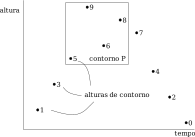
\includegraphics[scale=1]{cspace-5968}
    \label{fig:c-space5968}
  }
  \subfloat[contorno M e subconjunto O]{
    \includegraphics[scale=1]{cspace-7420}
    \label{fig:c-space7420}
  }

  \subfloat[contorno N]{
    \includegraphics[scale=1]{cspace-564}
    \label{fig:c-space564}
  }
  \caption{Espaço de contorno com diferentes contornos e subconjunto
    de contorno}
  \label{fig:c-space}
\end{figure}

Operações como retrogradação e rotação são semelhantes às realizadas
com alturas de notas. A retrogradação é obtida reordenando os
elementos de trás para frente. A rotação é obtida reordenando os
elementos de forma que os primeiros elementos do contorno são movidos
para o final. A rotação depende, além do contorno, de um fator que
determina quantos elementos são movidos para o fim. Por exemplo, uma
rotação de fator 1 tem o primeiro elemento movido para o final do
contorno. Uma rotação de fator 2 tem os 2 primeiros elementos movidos
para o fim, uma rotação de fator 3 tem os 3 primeiros elementos e
assim por diante.

Por exemplo, dado um contorno P(5 9 6 8) representado graficamente na
figura \ref{fig:operacoes-p} e aplicando-se retrogradação a este
contorno obtém-se como saída (8 6 9 5), ou seja
\verb!(retr(P(5 9 6 8)))! $\Rightarrow$ N(8 6 9 5) (figura
\ref{fig:operacoes-rp}). A operação de rotação de fator 1 aplicada a
este mesmo contorno P(5 9 6 8) retorna L(9 6 8 5), ou seja,
\verb!(rot(P(5 9 6 8)) 1)! $\Rightarrow$ L(9 6 8 5) (figura
\ref{fig:operacoes-rr1}). Aplicando-se a rotação de fator 2 a P(5 9 6
8) obtém-se M(6 8 9 5) (figura \ref{fig:operacoes-rr2}), e assim por
diante. O resultado de outras operações aplicadas ao contorno P(5 9 6
8) estão representadas graficamente na figura
\ref{fig:operacoes-simples}.

\begin{figure}
  \centering
  \subfloat[Contorno P]{
    \includegraphics{c-5968}
    \label{fig:operacoes-p}
  }
  \subfloat[Inversão de P]{
    \includegraphics{c-4031}
    \label{fig:operacoes-ip}
  }
  \subfloat[Retrógrado de P]{
    \includegraphics{c-8695}
    \label{fig:operacoes-rp}
  }
  \subfloat[Retrógrado da inversão de P]{
    \includegraphics{c-1304}
    \label{fig:operacoes-rip}
  }

  \subfloat[Rotação 1 de P]{
    \includegraphics{c-9685}
    \label{fig:operacoes-rr1}
  }
  \subfloat[Rotação 2 de P]{
    \includegraphics{c-6859}
    \label{fig:operacoes-rr2}
  }
  \subfloat[Rotação 3 de P]{
    \includegraphics{c-8596}
    \label{fig:operacoes-rr3}
  }
  \caption{Representação gráfica de operações simples com contorno P(5
  9 6 8)}
  \label{fig:operacoes-simples}
\end{figure}

A operação de expansão de intervalos é calculada multiplicando-se a
diferença entre os elementos do contorno pelo fator de expansão. Por
exemplo, a expansão de fator 2 do contorno P(5 9 6 8) é F(5 13 7
11). A diferença entre P$_1$ e P$_2$ é +4, entre P$_2$ e P$_3$ é -3, e
entre P$_3$ e P$_4$ é +2. Multiplicando-se estas diferenças pelo fator
de expansão 2 obtém-se +8, -6 e +4. Aplicando-se estas novas
diferenças ao contorno obtém-se que $F_2 = P_1$ + 8, ou seja, $F_2 = 5
+ 8$, então $F_2 = 13$. Aplicando-se este procedimento para calcular
os outros elementos obtém-se F(5 13 7 11).

A ordem de um contorno está relacionada com o número de elementos do
seu espaço de contorno. Pode-se subentender que o espaço ao qual um
contorno P(5 9 6 8) pertence contém outros elementos além destes
quatro contidos em P. Ou seja, pode-se afirmar que o espaço que
engloba P contém, além de 5, 9, 6 e 8, os elementos 0, 1, 2, 3, 4 e
7. Assim pode-se afirmar que o espaço de contorno de P contém pelo
menos 10 elementos. Dado apenas um contorno P(5 9 6 8) é impossível
saber se o espaço de contorno ao qual P pertence contém elementos além
do valor 9. Em um outro exemplo, o número de elementos do espaço de um
contorno V(1 2 4 5) contém certamente os elementos 0, 1, 2, 3, 4 e 5,
ou seja, 6 elementos. É impossível determinar se este espaço de
contorno contém elementos de valor maior que 5. Dessa forma a ordem de
um contorno pode ser sempre calculada somando o seu elemento de maior
valor com 1.

A operação de inversão de um contorno P de ordem $q$ é representada
por inv(P), e é matematicamente calculada por
$inv(P_n)=(q-1-P_n)$. Portanto, dado um contorno P(5 9 6 8), de ordem
10, $inv(P_0)=(10-1-P_0)$. Logo, $inv(P_0)=4$. Aplicando-se a mesma
operação aos outros elementos obtém-se o contorno
\verb!inv(P(5 9 6 8))!  $\Rightarrow$ S(4 0 3 1) (figura
\ref{fig:operacoes-ip}).

Relações de similaridade \cite{marvin.ea87:relating} são analisadas
com operações como comparação, matriz de comparação, forma prima e
classe de contorno.

A operação de comparação \tr{com(a,b)}\footnote{Operações como a
  função de comparação, a matriz de comparação e as diagonais da
  matriz de comparação são definidas em maiúsculas, ou seja,
  respectivamente COM, COM-Matrix e INT$_n$
  \cite{morris87:composition}. No entanto, como já foi visto, prefiro
  padronizar operações com minúsculas e nomes de contornos com
  maiúsculas.} retorna a diferença entre os valores de dois elementos
de contorno $a$ e $b$ considerando se um elemento tem valor maior,
igual ou menor que o outro. Em um contorno que mapeia a altura, esta
operação determina se um elemento é mais grave, mais agudo ou de mesma
altura que outro. Em um contorno que mapeia a densidade, a operação
determina se um elemento é mais, menos ou igualmente denso que o
outro. O resultado da operação de comparação é ``$+$'' se $b$ é maior
que $a$; ``$-$'' se $b$ é que $a$; e ``$0$'' se $b$ é igual a $a$. Por
exemplo, no contorno P(5 9 6 8), o valor de $com(P_0,P_1)$ é o sinal
``$+$'', o de $com(P_1,P_2)$ é ``$-$'', e o valor de $com(P_3,P_0)$ é
``$+$''. Esta medida de comparação pode ser invertida de modo que a
comparação entre dois elementos é igual ao inverso da comparação
destes elementos em ordem reversa. Esta idéia pode ser melhor
entendida observando-se a equação $com(a,b)=-com(b,a)$.

A matriz de comparação é bidimensional e compara um contorno com ele
próprio. Esta matriz mostra os resultados da operação de comparação
para todos os elementos de um contorno. Os contornos P, Q e R,
representados graficamente nas figuras \ref{fig:cseg-5968},
\ref{fig:cseg-5768} e \ref{fig:cseg-3051}, têm suas matrizes de
comparação nas figuras \ref{fig:matriz-5968}, \ref{fig:matriz-5768} e
\ref{fig:matriz-3051} respectivamente.

\begin{figure}
  \centering
  \subfloat[contorno P(5 9 6 8)]{
    \includegraphics{c-5968}
    \label{fig:cseg-5968}
  }
  \subfloat[contorno Q(5 7 6 8)]{
    \includegraphics{c-5768}
    \label{fig:cseg-5768}
  }
  \subfloat[contorno R(3 0 5 1)]{
    \includegraphics{c-3051}
    \label{fig:cseg-3051}
  }
  \caption{Representação gráfica dos contornos P, Q e R}
  \label{fig:repr-grafica-pqr}
\end{figure}

\begin{figure}
  \centering
  \subfloat[contorno P(5 9 6 8)]{
    \begin{tabular}{c|cccc}
      & $5$ & $9$ & $6$ & $8$ \\
      \hline
      $5$ & $0$ & $+$ & $+$ & $+$ \\
      $9$ & $-$ & $0$ & $-$ & $-$ \\
      $6$ & $-$ & $+$ & $0$ & $+$ \\
      $8$ & $-$ & $+$ & $-$ & $0$
    \end{tabular}
    \label{fig:matriz-5968}
  }
  \qquad
  \subfloat[contorno Q(5 7 6 8)]{
    \begin{tabular}{c|cccc}
      & $5$ & $7$ & $6$ & $8$ \\
      \hline
      $5$ & $0$ & $+$ & $+$ & $+$ \\
      $7$ & $-$ & $0$ & $-$ & $+$ \\
      $6$ & $-$ & $+$ & $0$ & $+$ \\
      $8$ & $-$ & $-$ & $-$ & $0$
    \end{tabular}
    \label{fig:matriz-5768}
  }
  \qquad
  \subfloat[contorno R(3 0 5 1)]{
    \begin{tabular}{c|cccc}
      & $3$ & $0$ & $5$ & $1$ \\
      \hline
      $3$ & $0$ & $-$ & $+$ & $-$ \\
      $0$ & $+$ & $0$ & $+$ & $+$ \\
      $5$ & $-$ & $-$ & $0$ & $-$ \\
      $1$ & $+$ & $-$ & $+$ & $0$
    \end{tabular}
    \label{fig:matriz-3051}
  }
  \caption{Exemplos de matriz de comparação}
  \label{fig:matriz-exemplos}
\end{figure}

As diagonais superiores paralelas à diagonal principal zero da matriz
de comparação são chamadas de int$_n$, onde $n$ é o número da
diagonal: 1 para a superior mais próxima da diagonal zero, 2 para a
seguinte, 3 para a posterior e assim por diante (figura
\ref{fig:int-exemplos}).

\begin{figure}
  \centering
  \subfloat[int$_1$]{
    \begin{tabular}{c|cccc}
      & $5$ & $9$ & $6$ & $8$ \\
      \hline
      $5$ &     & $+$ &     &     \\
      $9$ &     &     & $-$ &     \\
      $6$ &     &     &     & $+$ \\
      $8$ &     &     &     & 
    \end{tabular}
    \label{fig:int-1-5968}
  }
  \qquad
  \subfloat[int$_2$]{
    \begin{tabular}{c|cccc}
      & $5$ & $9$ & $6$ & $8$ \\
      \hline
      $5$ &     &     & $+$ &     \\
      $9$ &     &     &     & $-$ \\
      $6$ &     &     &     &     \\
      $8$ &     &     &     & 
    \end{tabular}
    \label{fig:int-2-5968}
  }
  \qquad
  \subfloat[int$_3$]{
    \begin{tabular}{c|cccc}
      & $5$ & $9$ & $6$ & $8$ \\
      \hline
      $5$ &     &     &     & $+$ \\
      $9$ &     &     &     &     \\
      $6$ &     &     &     &     \\
      $8$ &     &     &     & 
    \end{tabular}
    \label{fig:int-3-5968}
  }
  \caption{int$_n$ de matriz do contorno P(5 9 6 8)}
  \label{fig:int-exemplos}
\end{figure}

A diagonal int$_1$ retorna comparações entre os valores dos elementos
adjacentes do contorno. Por exemplo, em um contorno P(5 9 6 8),
int$_1=(+ - +)$ (figura \ref{fig:int-1-5968}), ou seja, no caso de
mapeamento de altura em função do tempo o movimento melódico é
ascendente entre 5 e 9, descendente entre 9 e 6, e ascendente entre 6
e 8. Esta comparação é feita também com uma operação conhecida como
série de contornos adjacentes (\tr{cas})\footnote{Em teorias de
  contornos não há consenso em relação a terminologia. Dessa forma há
  idéias semelhantes com nomes diferentes, como int$_1$ e série de
  contornos adjacentes \cite{friedmann87:response}. A série de
  contornos adjacentes de Friedmann, por exemplo, seria entendida por
  Morris como uma série de alturas de contorno adjacentes.}. A
operação de int$_2$ retorna a comparação entre elementos alternados do
contorno. Por exemplo, em P(5 9 6 8), int$_2=(+ -)$ (figura
\ref{fig:int-2-5968}), ou seja, a diferença entre 5 e 6 é positiva, e
entre 9 e 8 é negativa. A tabela \ref{tab:int-contornos} traz as
int$_n$ dos contornos P, Q e R, cujas matrizes são apresentadas nas
figuras \ref{fig:matriz-5968}, \ref{fig:matriz-5768} e
\ref{fig:matriz-3051} respectivamente.

\begin{table}
  \centering
  \begin{tabular}{r|ccc}
    Contorno & int$_1$ & int$_2$ & int$_3$ \\
    \hline
    P(5 9 6 8) & (+ - +) & (+ -) & (+) \\
    Q(5 7 6 8) & (+ - +) & (+ +) & (+) \\
    R(3 0 5 1) & (- + -) & (+ +) & (-)
  \end{tabular}
  \caption{Exemplos de int$_n$}
  \label{tab:int-contornos}
\end{table}

A forma normal de um contorno ocorre quando seus elementos aparecem em
ordem temporal de ocorrência, e com valores redefinidos de 0 (menor
valor) a $n-1$ (maior valor), onde n é o número de elementos do
contorno. O elemento de menor valor é redefinido para 0, o segundo
elemento de menor valor para 1, o terceiro para 2 e assim por
diante. Por exemplo, o contorno P(5 9 6 8) tem forma normal F(0 3 1
2), pois P$_0$, elemento de menor valor, é redefinido para 0, P$_2$,
segundo elemento de menor valor, para 1, P$_3$, terceiro de menor
valor, para 2, e P$_1$ para 3.  Esta operação de renumeração que
origina a forma normal\footnote{Friedmann define como classe de
  contorno o que Marvin define como forma normal.} é chamada
translação \cite[p. 228]{marvin.ea87:relating}.

%% falar da forma prima

A classe de contorno (\tr{cc}) é uma operação importante para a
verificação de similaridade entre contornos. Obtém-se a classe de
contorno numerando-se ordenadamente todas as alturas de contorno de
$0$ a $(n-1)$, sendo $n$ o número total de alturas de contorno do
contorno. Uma classe de contorno engloba todos os contornos
considerados equivalentes. Dois ou mais contornos são considerados
equivalentes quando geram uma mesma matriz de comparação, ou seja,
quando mantêm a mesma estrutura de registro entre suas notas. Dessa
forma, dado um contorno P(5 9 6 8), são considerados seus equivalentes
os contornos (1 5 2 3), (0 10 4 7), (0 3 1 2) e muitos outros. Todos
eles têm (0 3 1 2) como forma normal e classe de contorno. A função de
similaridade (\tr{csim}) mede numericamente o grau de semelhança entre
dois contornos de mesma cardinalidade. O maior nível de similaridade
entre contornos tem valor 1 e o menor tem valor 0. Este número é
calculado comparando-se o triângulo superior da matriz de comparação
dos dois contornos. Atribui-se o valor 1 para cada posição da matriz
cujo símbolo é o mesmo no triângulo superior das duas matrizes. O
valor de similaridade é o quociente da soma dessas equivalências pelo
número total de posições do triângulo superior.

A função de similaridade pode ser melhor compreendida por meio dos
exemplos da figura \ref{fig:triangulos-com-matrix} e tabela
\ref{tab:similaridade-contornos}. As figuras \ref{fig:triangulo-5968},
\ref{fig:triangulo-5768} e \ref{fig:triangulo-3051} mostram os
triângulos superiores das matrizes de comparação dos contornos P(5 9 6
8), Q(5 7 6 8) e R(3 0 5 1), respectivamente. As figuras
\ref{fig:triangulo-pq}, \ref{fig:triangulo-pr} e
\ref{fig:triangulo-qr} mostram as semelhanças entre os triângulos
superiores das matrizes de comparação dos contornos P e Q, P e R, e Q
e R respectivamente. Entre P e Q há 5 elementos semelhantes entre os 6
possíveis no triângulo. Dessa forma a função de similaridade entre P e
Q é $5/6$, ou csim(P,Q)$=0,83$. Entre P e R há apenas um elemento
semelhante entre 6 possíveis. Assim, csim(P,R)$=0,16$. A tabela
\ref{tab:similaridade-contornos} mostra os valores de csim entre estes
contornos.

\begin{figure}
  \centering
  \subfloat[contorno P(5 9 6 8)]{
    \begin{tabular}{c|cccc}
      & $5$ & $9$ & $6$ & $8$ \\
      \hline
      $5$ &     & $+$ & $+$ & $+$ \\
      $9$ &     &     & $-$ & $-$ \\
      $6$ &     &     &     & $+$ \\
      $8$ &     &     &     &
    \end{tabular}
    \label{fig:triangulo-5968}
  }
  \qquad
  \subfloat[contorno Q(5 7 6 8)]{
    \begin{tabular}{c|cccc}
      & $5$ & $7$ & $6$ & $8$ \\
      \hline
      $5$ &     & $+$ & $+$ & $+$ \\
      $7$ &     &     & $-$ & $+$ \\
      $6$ &     &     &     & $+$ \\
      $8$ &     &     &     & 
    \end{tabular}
    \label{fig:triangulo-5768}
  }
  \qquad
  \subfloat[contorno R(3 0 5 1)]{
    \begin{tabular}{c|cccc}
      & $3$ & $0$ & $5$ & $1$ \\
      \hline
      $3$ &     & $-$ & $+$ & $-$ \\
      $0$ &     &     & $+$ & $+$ \\
      $5$ &     &     &     & $-$ \\
      $1$ &     &     &     & 
    \end{tabular}
    \label{fig:triangulo-3051}
  }

  \subfloat[P x Q]{
    \begin{tabular}{c|cccc}
      &     &     &     &     \\
      \hline
      &     & $+$ & $+$ & $+$ \\
      &     &     & $-$ &     \\
      &     &     &     & $+$ \\
      &     &     &     &
    \end{tabular}
    \label{fig:triangulo-pq}
  }
  \qquad
  \subfloat[P x R]{
    \begin{tabular}{c|cccc}
      &     &     &     &     \\
      \hline
      &     &     & $+$ &     \\
      &     &     &     &     \\
      &     &     &     &     \\
      &     &     &     &
    \end{tabular}
    \label{fig:triangulo-pr}
  }
  \qquad
  \subfloat[Q x R]{
    \begin{tabular}{c|cccc}
      &     &     &     &     \\
      \hline
      &     &     & $+$ &     \\
      &     &     &     & $+$ \\
      &     &     &     &     \\
      &     &     &     &
    \end{tabular}
    \label{fig:triangulo-qr}
  }
  \caption{Triângulos superiores de matrizes de comparação}
  \label{fig:triangulos-com-matrix}
\end{figure}

\begin{table}
  \centering
    \begin{tabular}{c|ccc}
      & (5 9 6 8) & (5 7 6 8) & (3 0 5 1) \\
      \hline
      (5 9 6 8) & 1 & .83 & .16 \\
      (5 7 6 8) & .83 & 1 & .33 \\
      (3 0 5 1) & .16 & .33 & 1
    \end{tabular}
    \caption{Similaridade entre contornos}
  \label{tab:similaridade-contornos}
\end{table}

Os intervalos de contorno (\tr{ci})\footnote{Friedmann utiliza
  maiúsculas para definir todas as suas operação com
  maiúsculas. Utiliza CC, CI, CIA, CCV, etc.} representam as relações
entre alturas de contorno de uma classe de contorno e podem ser
entendidos de duas formas: guardando o valor entre as alturas de
contorno \cite{friedmann85:methodology}, ou guardando apenas a
direção, mas não o valor da diferença entre as alturas de contorno
\cite{morris93:directions}. Por exemplo, para um mesmo contorno P(0 3
1 2), o intervalo de contorno entre $P_1$ e $P_2$ para Friedmann é -2,
e para Morris, ``$-$''.

O vetor de intervalos de contornos (\tr{cia}) descreve a freqüência de
cada tipo de intervalo de contorno em uma classe de contorno. Por
exemplo, o contorno P(0 3 1 2) tem vetor de intervalos de contornos
(2,1,1/1,1,0). Os dígitos à esquerda da barra representam os
intervalos de contorno ascendentes em ordem crescente, e os dígitos à
direita os intervalos de contorno descendentes em ordem crescente de
valor absoluto. \cite{friedmann85:methodology}. Dessa forma, neste
contorno P(0 3 1 2) há 2 intervalos de valor +1, 1 intervalo de valor
+2 e outro intervalo de valor +3. Além disso há um intervalo de valor
-1, outro intervalo de valor -2 e nenhum intervalo de valor -3. Os
vetores de classe de contorno (\tr{ccvi} e \tr{ccvii}), de dois
dígitos cada um, refletem os movimentos ascendentes e descendentes de
um contorno e são calculados a partir dos intervalos de contorno
ascendentes e descendentes.

A redução de contornos é possível a partir de dois diferentes
algoritmos \cite{adams76:melodic,morris93:directions}. O algoritmo de
Adams, criado para definir uma tipologia de contornos, reduz uma
melodia inteira a apenas quatro alturas de contorno\footnote{Adams
  utiliza uma terminologia diferenciada da que apresento aqui.}: a
primeira altura, a última, a mais aguda e a mais grave. O algoritmo de
Morris, processado em várias etapas, reduz a melodia através da
observação de mudanças de direção entre segmentos adjacentes e
eliminação de alturas de contorno.

%% o que é a tipologia de adams?
A tipologia de Adams considera a inclinação entre as quatro alturas de
contorno extremas e compreende 15 tipos de contornos melódicos, como
se vê na figura \ref{fig:adams-typology}. A inclinação entre a nota
inicial e final é indicada por $S1$ ($I > F$), $S2$ ($I = F$) e $S3$
($I < F$). A mudança de direção é indicada por $Dø$ (sem mudança de
direção), $D1$ (se H ou L são diferentes de I ou F) e $D2$ (se H e L
são diferentes de I e F). A ordem entre as mudanças de direção,
chamada \eng{reciprocal}, é indicada por $R1$ (H antes de L) e $R2$ (L
antes de H) \cite{adams76:melodic}.

\begin{figure}
  \centering
  \includegraphics[scale=.6]{adams-typology}
  \caption{Tipologia de contornos de Charles Adams}
  \label{fig:adams-typology}
\end{figure}

O estado de arte das teorias de contornos aqui relacionadas vem sendo
elevado através da implementação de novos conceitos e operações, e da
constante revisão crítica de autores como Beard e Clifford
\cite{beard03:contour,clifford95:contour}. O principal objetivo desta
revisão de teorias de contornos é reunir e conhecer operações de
contornos para testar suas funcionalidades em aplicações na área de
Composição Musical.

\chapter{Ferramentas computacionais}
\label{cha:ferramentas}

Para este trabalho desenvolvi ferramentas computacionais exclusivas
como o software para processamento de contornos Goiaba. Utilizei a
plataforma Linux para desenvolver todo o trabalho, pois além de ser
livre, com ela é possível concatenar programas. Com o Linux é possível
desenvolver funções que enviem a saída de dados de um programa como o
Goiaba para a entrada de dados de outro programa como o editor de
partituras Lilypond (vide seção \ref{sec:lilypond}), ou usar
bibliotecas de gráficas para criar interfaces para o usuário. Com essa
conectividade posso desenvolver um software mais completo sem precisar
necessariamente desenvolver bibliotecas ou programas já existentes.

\section{Goiaba, um software para processar contornos}
\label{sec:goiaba-software-para}

O \goiaba{}\footnote{Assim como ocorreu com o nome da empresa de
  computadores \eng{Apple} em sua fundação, não houve uma razão
  especial para dar ao software desenvolvido neste trabalho o nome
  Goiaba.} é um software desenvolvido na linguagem Common Lisp
\cite{graham94:lisp,seibel05:practical,shapiro92:common}, o compilador
SBCL \cite{team07:sbcl} e com metodologia \eng{bottom-up}. Utilizo no
desenvolvimento do \goiaba{} ferramentas como GNU Emacs
\cite{stallman07:gnu} e Slime \cite{team05:slime}.

A metodologia \eng{bottom-up} utilizada está relacionada à direção do
desenvolvimento, a partir de subsistemas mais simples em direção ao
programa como um todo. Ela é bastante adequada ao desenvolvimento de
programas que progressivamente têm sua complexidade
aumentada. Programas como \TeX{}\footnote{Sistema de
  tipografia. Disponível em \url{www.tug.org}.} e X
Windows\footnote{Sistema gráfico de janelas do Linux. Disponível em
  \url{www.x.org}.} têm sido desenvolvidos dessa forma
\cite[p. vi]{graham94:lisp}. Esta metodologia tem vantagens como a
possibilidade de deixar os programas menores e mais ágeis, de
reutilizar funções de um subsistema em outro, de simplificar a leitura
dos programas e de clarear as idéias do programador
\cite[p. 4]{graham94:lisp}.

O \goiaba{} tem as classes \texttt{ponto}, \texttt{contorno-simples} e
\texttt{contorno-duracao}. A classe \texttt{ponto} define as alturas
de contorno no tempo como pontos cartesianos como (x, y), onde x é o
tempo e y a altura. A classe \texttt{contorno-duracao} define um
contorno como uma lista de pontos como ((x, y) (z, w)), e a classe
\texttt{contorno-simples} define contornos apenas com as alturas como
(y w).

Algumas macros de leitura foram definidas para simplificar o processo
de criar instâncias de objetos. Por exemplo, para criar uma instância
do tipo \texttt{ponto} pode-se fazer normalmente
\texttt{(make-instance 'ponto :x 0 :y 3)} ou simplesmente
\verb!#p(0 3)! com a macro de leitura. Da mesma maneira, um
\texttt{contorno-duracao} com dois pontos pode ser instanciado com
\verb!#d(#p(0 3) #p(1 4))! ao invés de usar \texttt{make-instance}.

Contornos são representados simbolicamente de duas maneiras: como
contornos simples, considerando apenas as alturas de contorno
\verb!(5 9 6)!, e como contornos com duração, considerando também o
local no tempo onde ocorre cada altura de contorno:
\verb!((0 5)(1 9)(2 6))!. Apesar de ter uma codificação específica que
comporte a influência do tempo no contorno, ainda não estou
trabalhando com este elemento.

As operações em contornos são implementadas em métodos, aproveitando
do despacho múltiplo usado pelo sistema de objetos de Common Lisp
(CLOS). Desse modo um método como \texttt{transpor} se comporta de
maneira diferente dependendo qual o tipo do seu primeiro parâmetro:

\begin{verbatim}
(defmethod transpor ((objeto contorno-duracao) fator)
  (map-contorno-duracao #L(transpor !1 fator) (pontos objeto)))

(defmethod transpor ((objeto contorno-simples) fator)
  (map-contorno-simples #L(+ !1 fator) (pontos objeto)))
\end{verbatim}

\goiaba{} tem diversas operações para lidar com contornos, como
tranposição, inversão, retrogradação, rotação e expansão de
intervalos. Além disso operações definidas na literatura também estão
implementadas, como redução de contornos \cite{adams76:melodic},
classe de contorno, série de contornos adjacentes, vetor de séries de
contornos adjacentes, intervalo de contorno, vetor de intervalo de
contorno, vetor de classe de contorno I e II
\cite{friedmann85:methodology} e matriz de comparação
\cite{morris93:directions}.

Finalmente, \goiaba{} usa a biblioteca
Cl-pdf\footnote{www.cliki.net/CL-PDF} para plotar facilmente contornos
definidos, permitindo a fácil visualização de operações em contornos.
Por exemplo, o código seguinte gera um gráfico com o contorno
original, sua transposição, retrogradação, inversão, rotação,
ampliação de altura e inserção de ponto (figura
\ref{fig:operacoes}). Neste exemplo defino o contorno \verb!c1!, o
arquivo no qual o gráfico será criado, as dimensões do gráfico e as
operações e cores que serão geradas no gráfico.

\begin{verbatim}
(let ((c1 #d(#p(0 0) #p(1 5) #p(2 3) #p(3 4) #p(4 1) #p(5 3))))
  (plot-page "contornos.pdf"
    (plot-contorno-full 50 500
                        c1 "original" :red
                        (transpor c1 2) "transposição" :green
                        (retrogradar c1) "retrógrado" :blue
                        (inverter c1) "inversão" :pink
                        (aumentar-altura c1 2) "aumentar-altura" :lightblue
                        (rotacionar c1 1) "rotação" :darkcyan
                        (insere-ponto c1 '(1 3) 2) "insere ponto" :purple)))
\end{verbatim}

\begin{figure}
  \centering
  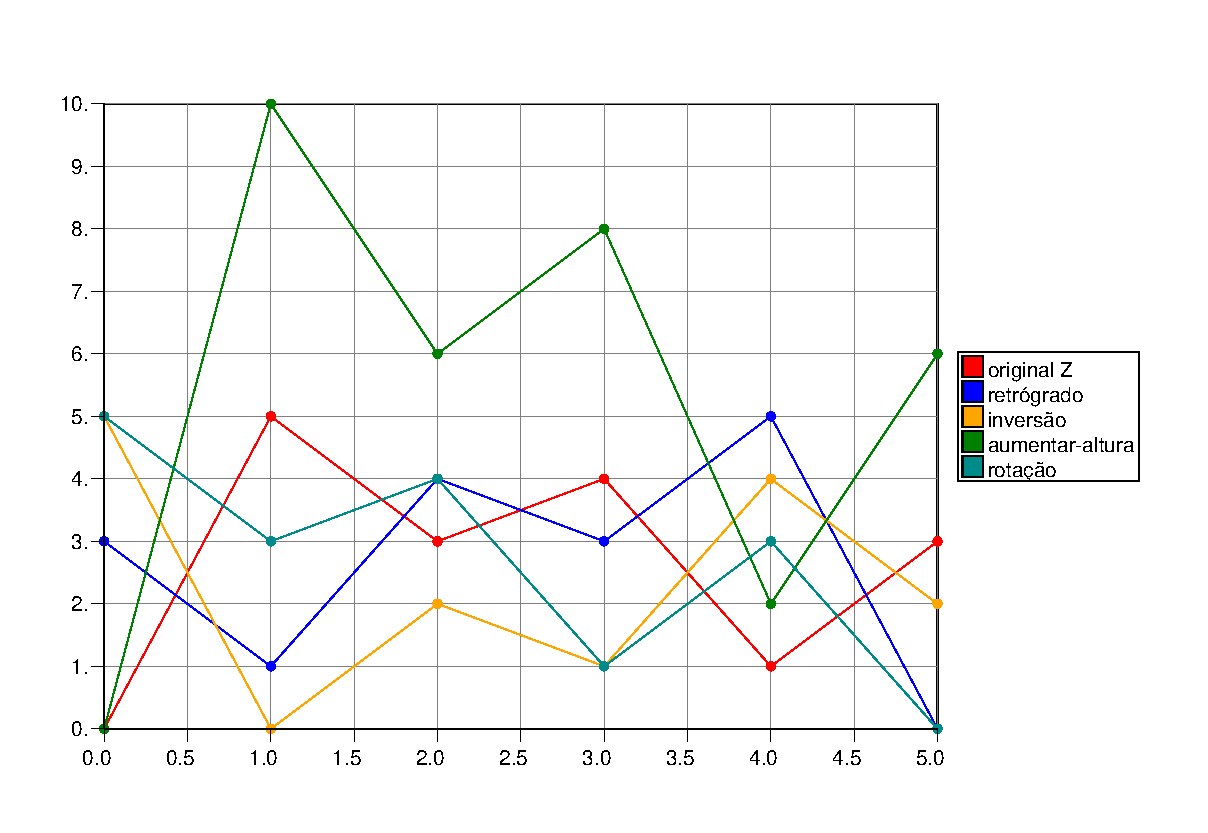
\includegraphics[scale=.5]{contornos}
  \caption{Operações em contorno (0 5 3 4 1 3)}
  \label{fig:operacoes}
\end{figure}

Para o futuro pretendo implementar a possibilidade de gerar contornos
a partir de partituras musicais e vice-versa e implementar uma
interface gráfica. O desenvolvimento do \goiaba{} segue procedimentos
oriundos do desenvolvimento de software livre como uso de controle de
versão e disponibilização do código-fonte na
internet\footnote{Disponível como marcos-mestrado.git em
  \url{git.genos.mus.br}.}.

As descrições das teorias de contornos nem sempre são feitas pelos
seus autores de uma forma totalmente clara. A programação de uma
teoria em um software de computador é um exercício poderoso no
processo de aprendizagem, pois o programador é obrigado a expressar de
forma precisa a compreensão que tem de uma idéia obscura. Dessa forma
a implementação das operações de contorno em um software de computador
ajuda na compreensão da teoria, uma vez que é preciso entender
totalmente como cada operação se processa e que funcionalidade tem
para implementá-las.

As operações são implementadas como funções. Para isso é necessário
conhecê-las de modo profundo e abstraí-las precisamente em descrições
matemáticas. As funções têm que ser testadas a partir de aplicações
práticas. Para os testes são utilizados exemplos originais dos
autores, e são criados exemplos adicionais, o que ajuda na compreensão
da funcionalidade de cada operação. Finalmente combinações de funções
são observadas e testadas. Este processo de aprendizagem tem se
mostrado muito eficiente e se tornou fundamental para o
desenvolvimento da pesquisa.

\section{Outras ferramentas computacionais}
\label{sec:outr-ferr-comp}

Neste trabalho além de desenvolver o Goiaba utilizo o Lilypond tanto
para gerar partituras através do Goiaba quanto para escrever a obra
\obra{}. Uso também o sistema de controle de versão Git que ajudou no
desenvolvimento do Goiaba, na composição da obra e na comunicação de
dados com o orientador.

Além disso essas ferramentas utilizadas são aqui descritas porque,
apesar de serem amplamente utilizadas em outras áreas como ciência da
computação ou matemática, são praticamente desconhecidas entre
músicos.

\subsection{Lilypond}
\label{sec:lilypond}

O Lilypond \cite{nienhuys.ea08:lilypond} é um software livre para
edição automática de partituras. É automático porque na maioria dos
casos dispensa ajustes como número de compassos por sistema, número de
sistemas por página, distância entre pentagramas, entre notas e
acidentes, entre outros.

O Lilypond processa música descrita em uma sintaxe própria de marcação
e gera arquivos como .pdf, .ps, .midi, .png, .svg entre outros. A
figura \ref{fig:exemplo-lily} por exemplo é gerada com um código como
\verb!{ \clef bass c4 d8 e d4 c }!. É possível utilizar variáveis para
abstrair códigos. Em Composição isso pode ser usado para abstrair
motivos, por exemplo. Dessa forma, um código como este:

\begin{verbatim}
{
  c4 e
  e16 d c d
  d4 fis
  e16 d c d
}
\end{verbatim}

pode ter os motivos abstraídos em variáveis e ser escrito assim:

\begin{verbatim}
motivoA = { c4 e }
motivoB = { e16 d c d }
{
  \motivoA
  \motivoB
  \transpose c d {\motivoA}
  \motivoB
}
\end{verbatim}

\begin{figure}
  \centering
  \includegraphics{exemplo-lily}
  \caption{Partitura gerada no Lilypond}
  \label{fig:exemplo-lily}
\end{figure}

O Lilypond ainda se relaciona com o \LaTeX{}\footnote{Sintaxe de
  marcação de documentos e um sistema livre e automático de preparação
  de documentos.} e OpenOffice\footnote{Pacote com softwares livres de
  escritório como editor de texto e planilha de cálculos.} de modo a
simplificar a produção de exemplos musicais para inserir em texto. Por
fim é possível desenvolver programas que usem o Lilypond para gerar
partitura automaticamente. O Rameau, por exemplo, faz análise
harmônica automática e gera como saída partitura através do Lilypond
\cite{kroger08:rameau}.

\subsection{Git}
\label{sec:git}

%% dizer o que é um sistema de controle de versão
Um sistema de controle de versão é um programa de computador que tem
como função gerenciar todas as versões de arquivos de um determinado
projeto. É normalmente utilizado em desenvolvimento de software,
embora seu uso não seja restrito a este tipo de atividade.

%% falar de funcionalidades de um sistema de controle de versão
Um sistema de controle de versão possibilita o trabalho colaborativo
sem conflitos entre as versões dos arquivos dos participantes. Com um
sistema deste é possível comparar versões de arquivos para observar as
mudanças, voltar a versões antigas para encontrar erros, criar novos
ramos paralelos de desenvolvimento e outras inúmeras funcionalidades.

%% explicar em linhas gerais como um sistema de controle de versão funciona
Normalmente inicia-se o controle de versão no diretório raiz de um
projeto. O sistema cria um repositório oculto para onde são copiados
todos os arquivos e mudanças colocados em controle de versão. O
procedimento do usuário normalmente é salvar cada mudança feita em um
arquivo com um título e descrição, de forma que ele possa reconhecer a
mudança quando precisar. A figura \ref{fig:controle-de-versao} mostra
um esquema gráfico deste processo. Neste exemplo o arquivo foo é
alterado e a linha com o texto \verb!43! é substituída por
\verb!43 MS!. O sistema compara a versão do diretório com a versão do
repositório e salva apenas as mudanças. O esquema de funcionamento
interno dos repositórios é diferente em cada sistema de controle de
versão, embora o processo para o usuário seja sempre parecido com o
que apresentamos.

\begin{figure}
  \centering
  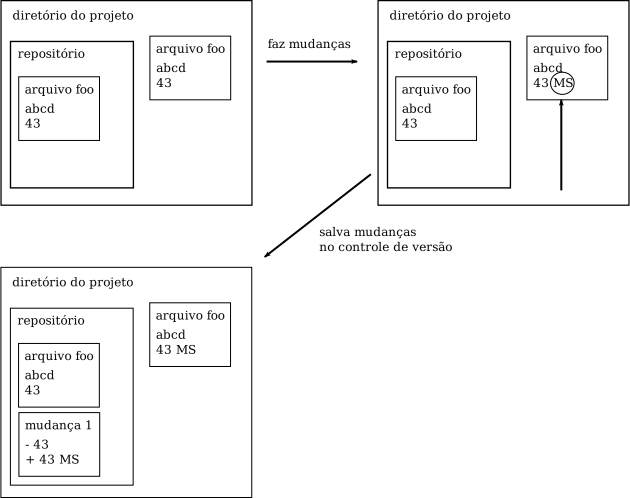
\includegraphics[scale=.6]{controle-de-versao}
  \caption{Funcionamento de um sistema de controle de versão}
  \label{fig:controle-de-versao}
\end{figure}

%% desenvolver sobre git
O Git\footnote{\url{http://git.or.cz}} é um software livre de controle
de versão bastante poderoso e veloz. O Git permite um desenvolvimento
distribuído, em que cada desenvolvedor pode ter uma cópia local do
repositório central, que fica acessível via SSH\footnote{Protocolo de
  acesso remoto seguro} ou HTTP. O Git tem suporte a desenvolvimento
não-linear com ramos, ou seja, é possível desenvolver uma nova versão
de um programa ao mesmo tempo em que defeitos da versão anterior são
corrigidos. Com o Git é possível trabalhar com grandes projetos e ter
velocidade de processamento muito maior que outros sistemas de
controle de versão. O Git proporciona segurança do histórico de
mudanças. Uma vez que uma mudança é registrada ela pode ser revertida,
mas não pode ser removida do histórico, ou seja, é possível saber tudo
que foi feito em um projeto. Finalmente o Git oferece um conjunto de
ferramentas de fácil utilização para gerenciar o projeto. A figura
\ref{fig:historico-git} mostra uma interface gráfica do Git para
visualizar histórico de mudanças, autor, data e hora da mudança,
arquivos alterados e a alteração em si.

\begin{figure}
  \centering
  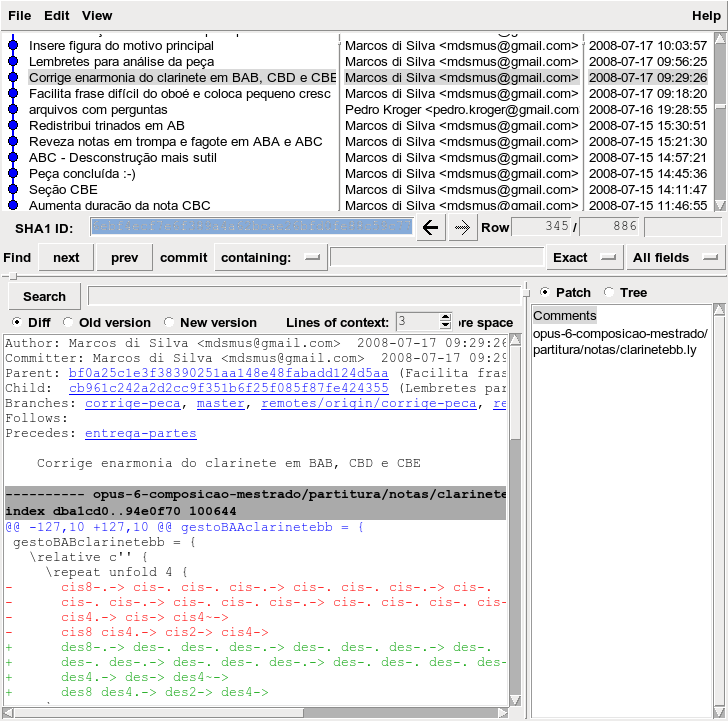
\includegraphics[scale=.62]{figura-base-gitk}
  \caption{Visualização de histórico do projeto no Gitk}
  \label{fig:historico-git}
\end{figure}

%% falar sobre controle de versão neste trabalho (programa, projeto,
%% composições e dissertação)
Utilizo o sistema de controle de versão Git no desenvolvimento de todo
o trabalho. Mantive este projeto em um repositório
central\footnote{Disponível em
  \url{git.genos.mus.br/?r=marcos-mestrado}.} com acesso irrestrito ao
autor e orientador. Este procedimento dinamizou muito o trabalho uma
vez que todo e qualquer comentário ou modificação pôde ser feita
diretamente no texto sem necessidade de um aviso prévio. O sistema de
controle de versão foi suficiente para registrar dados como mudança e
autoria. Uso controle de versão no gerenciamento do desenvolvimento do
Goiaba, nos experimentos composicionais, na obra final, e na escrita
desta dissertação e do seu projeto.

A possibilidade de criar ramos diferentes de desenvolvimento nos
possibilitou fazer a refatoração do Goiaba ao mesmo tempo que podíamos
ter em funcionamento uma versão estável anterior.

Na composição o sistema possibilitou, por exemplo, consultas
posteriores a fragmentos que havia desistido de manter na obra. Com um
sistema deste tipo é possível reconstituir o passo-a-passo do
compositor na criação de uma obra musical.

A produção desta dissertação ilustra o uso de controle de versão em um
projeto colaborativo. Em um trabalho sem este tipo de ferramenta,
enquanto o orientador faz notas no texto, o autor não pode editá-lo
para não criar conflitos entre as versões. Neste trabalho pudemos
trabalhar sempre simultaneamente.

\chapter{Análise da obra \obra{}}
\label{cha:anal-da-obra}
%% falar de contornos, motivos, forma, altura, timbre, gestual

A obra \obra{} é um quinteto de madeiras em movimento único. Sua
composição foi focada no uso sistemático de contornos melódicos e
não-melódicos. Além de contornos, trabalhei com proporções, metas
composicionais, gestos e motivos em um nível secundário.

A obra contém três elementos musicais a partir dos quais todo o
material composicional é derivado. O primeiro elemento é uma estrutura
de duas vozes---representada pela figura \ref{fig:bifonia}. O segundo
elemento é o motivo $\alpha$\footnote{Os motivos são descritos na
  seção \ref{sec:uso-de-motivos}.}, o principal da obra, representado
pela figura \ref{fig:motivo-alfa}. Este motivo é derivado por meio de
alternância entre as notas da estrutura de duas vozes. O terceiro
elemento é o contorno principal da peça \contpr{}, representado pela
figura \ref{fig:534120}. Este é o contorno do motivo $\alpha$.

\begin{figure}
  \centering
  \subfloat [Estrutura de duas vozes]{
    \includegraphics{bifonia}
    \label{fig:bifonia}
  }
  \subfloat [Motivo $\alpha$]{
    \includegraphics{motivo-alfa}
    \label{fig:motivo-alfa}
  }

  \subfloat [Representação gráfica do contorno (5 3 4 1 2 0)]{
    \includegraphics{c-534120}
    \label{fig:534120}
  }
  \caption{Elementos geradores}
  \label{fig:elementos-geradores}
\end{figure}

\section{Aspectos formais}
\label{sec:aspectos-formais}

Esta obra pode ser dividida em sete seções. Cada uma destas seções
contém uma textura característica, um desenho gestual e uma meta
composicional.
%% reescrever período
O tamanho de cada seção foi definido no planejamento inicial da obra
com proporções baseadas na razão áurea.
%%
Porém, como admito uma tolerância relativamente alta entre
planejamento e resultado final, estas proporções ficaram diferentes na
versão final da obra.
%% dizer o quanto desviei
Admiti esta alta tolerância porque decidi concentrar esforços no
objetivo principal do trabalho e deixar questões como proporções
formais em segundo plano.

A tabela \ref{tab:secoes-obra} contém informações de cada uma das
seções da obra como a duração, andamento, a localização do seu início
e fim pelo número de compasso e letra de ensaio.

\begin{table}
  \centering
  \begin{tabular}{r|ccccccc}
    Seção & 1 & 2 & 3 & 4 & 5 & 6 & 7 \\
    \hline
    Início (letra ensaio) & - & E & H & L & O & R & U \\
    Início (comp.) & 1 & 37 & 57 & 105 & 134 & 173 & 215 \\
    Final (comp.) & 36 & 56 & 104 & 133 & 172 & 214 & 244 \\
    Duração aprox. (s) & 132 & 91 & 108 & 56 & 87 & 23 & 16\\
    Andamento M.M & 82 & 66 & 120 & 120 & 108 & 112 & 112 \\
  \end{tabular}
  \caption{Seções formais da obra}
  \label{tab:secoes-obra}
\end{table}

\subsection{Planejamento da composição}
\label{sec:plan-da-comp}

O planejamento inicial desta peça foi feito pouco menos de um ano
antes de sua composição. Neste planejamento detalho elementos de alto
nível de abstração como forma, seções, microseções, proporções,
andamentos, metas composicionais e texturas. Considero estruturas
musicais como temas, movimentos, seções como de alto nível de
abstração, e notas e durações como de baixo nível de abstração. O
resultado deste planejamento pode ser visto na tabela
\ref{tab:planejamento-inicial}. Muitos dos elementos planejados foram
modificados em função da própria dinâmica da composição. À medida que
a música foi criada adaptei o planejamento privilegiando o resultado
artístico.

\begin{table}
  %% aumentar a fonte das palavras
  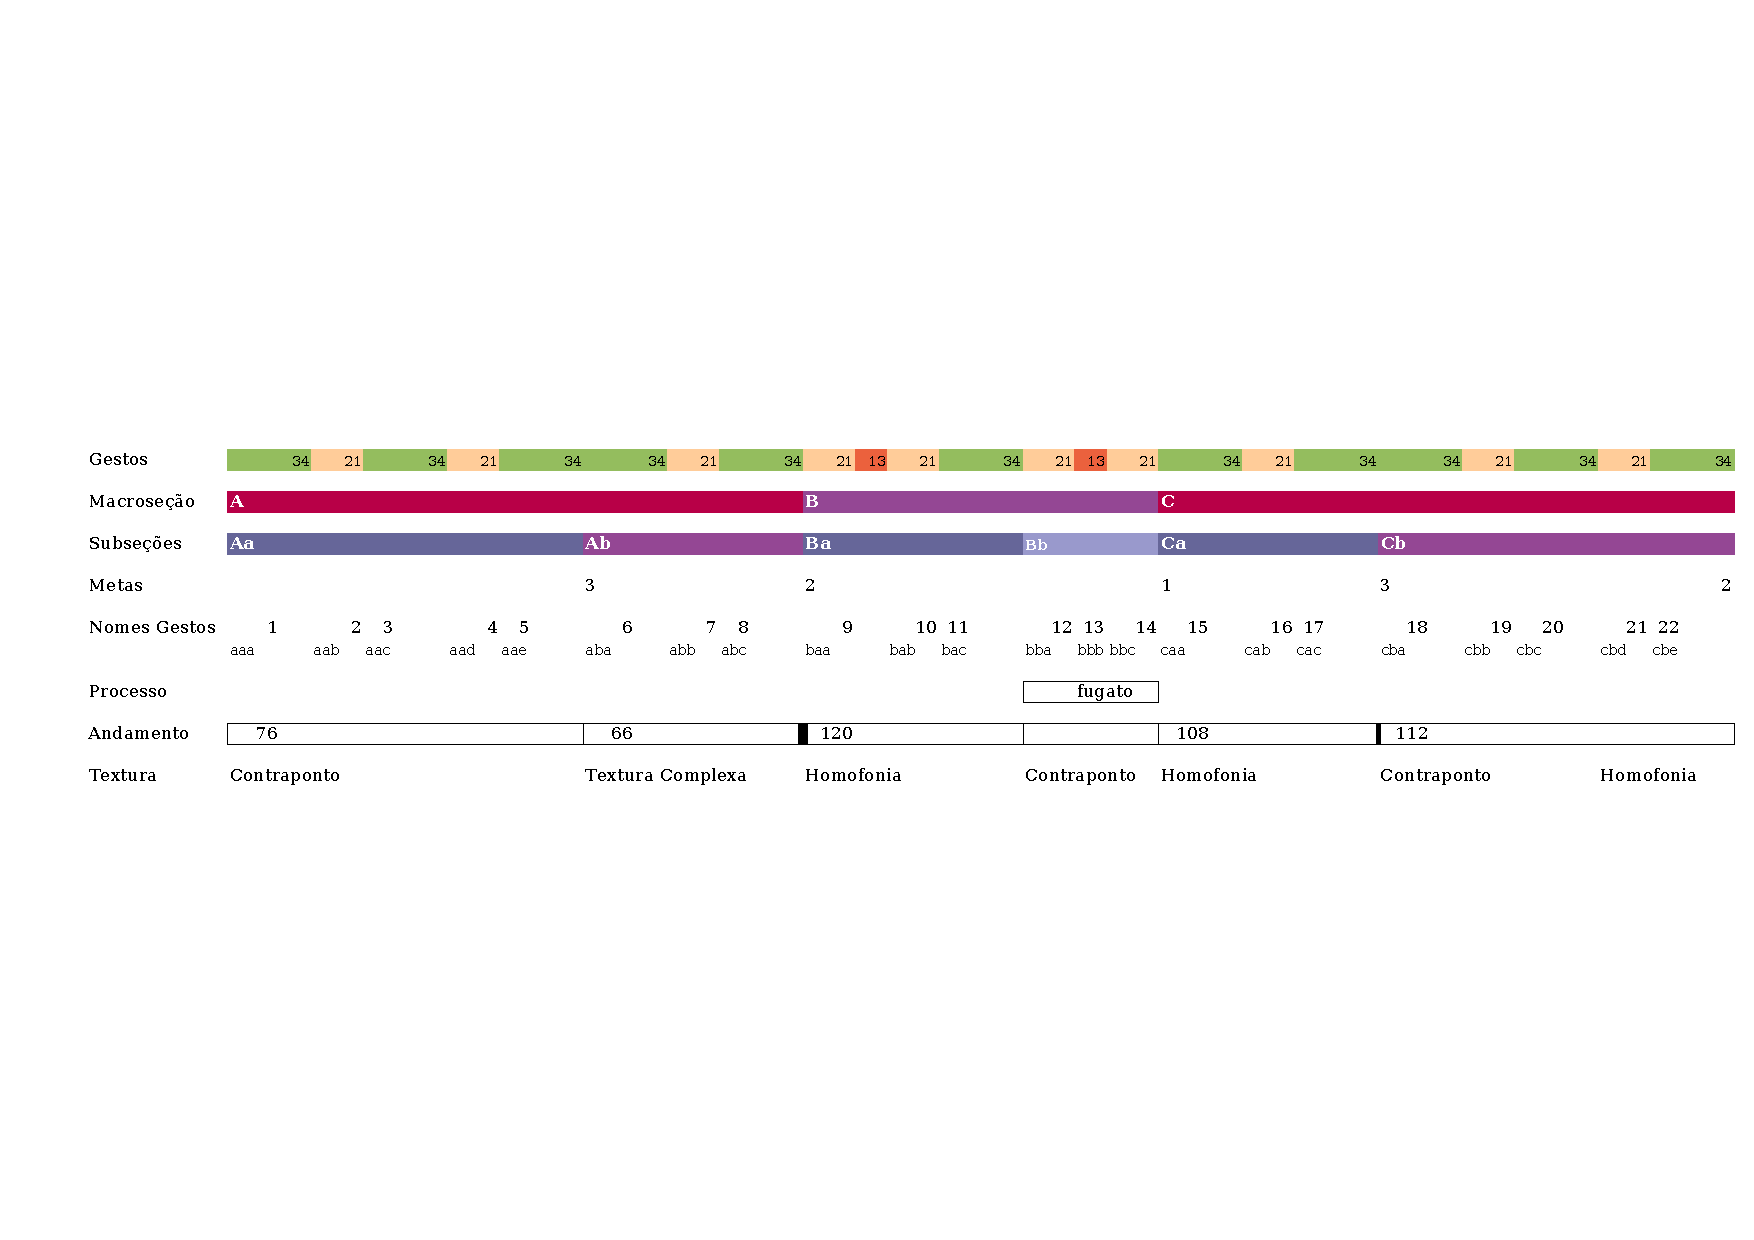
\includegraphics[scale=.81]{planejamento-inicial}
  \caption{Planejamento inicial da peça}
  \label{tab:planejamento-inicial}
\end{table}

No planejamento previ criar seis seções agrupáveis duas a duas (Aa,
Ab, Ba, Bb, Ca, Cb). Durante a composição dividi a seção Cb em dois
pedaços, criando então uma nova seção.

As seções menores estão desmembradas em sub-seções (Aaa, Aab, Aac e
assim por diante). Estas divisões mínimas foram planejadas para conter
microgestos, mas ao longo do processo preferi trabalhar com gestos
maiores e usá-las para marcar mudanças de instrumental, de timbre, ou
outras intervenções musicais. Além disso os nomes e as numerações dos
gestos ajudaram na organização dos arquivos do Lilypond durante a
composição.

O uso destas microseções para mudança de instrumental pode ser visto
na seção inicial da peça (vide tabela
\ref{tab:microsecoes-primeira-secao}). A microseção \textbf{Aaa}
(compassos 1--8) compreende o solo do fagote e tem 29 segundos. a
microseção \textbf{Aab} (compassos 9--14) compreende o trio entre
fagote, clarinete e oboé e tem 22 segundos. A microseção \textbf{Aac}
(compassos 15--22), de 29 segundos compreende o duo entre a melodia
inicial no clarinete e o contraponto da flauta. A microseção
\textbf{Aad} (compassos 23--28), de 22 segundos compreende o quinteto
completo. Por último, a microseção \textbf{Aae} (compassos 29--36), de
29 segundos, compreende o quarteto fl./ob./cal./fg. e o aumento da
densidade.

\begin{table}
  \centering
  \begin{tabular}{r|rrrrr}
    & Aaa & Aab & Aac & Aad & Aae \\
    \hline
    Flauta & & & \cinzaa & \cinzaa & \cinzaa \\
    Oboé & & \cinzab & & \cinzab & \cinzab \\
    Clarinete & & \cinzaa & \cinzaa & \cinzaa & \cinzaa \\
    Trompa & & & & \cinzaa & \cinzaa \\
    Fagote & \cinzab & \cinzab & & \cinzab &
  \end{tabular}
  \caption{Instrumentos utilizados na primeira seção}
  \label{tab:microsecoes-primeira-secao}
\end{table}

%% explicar melhor este período:
Os números 1, 2 e 3 associados às metas representam seu grau de
importância na peça.
%% verificar: gradação ou graduação
Tal graduação porém não foi implementada. Os andamentos foram
levemente modificados para adequação ao material de cada seção. Na
tabela \ref{tab:planejamento-inicial} as barras mais grossas nos
campos dos andamentos representam silêncio entre as seções e não foram
implementadas na versão final. As texturas planejadas foram mantidas
exceto pela seção planejada C (seções 5--7). Neste ponto não há de
fato textura homofônica.

\subsection{Descrição das seções}
\label{sec:descricao-das-secoes}

A seção 1, no início da obra\footnote{Vide seções na tabela
  \ref{tab:secoes-obra}.}, contém em toda sua extensão a repetição de
uma mesma melodia (figura \ref{fig:melodia-inicial}). Esta repetição é
alternada entre os instrumentos. Ainda nesta seção, a partir do
compasso 9, o motivo $\alpha$ (figura \ref{fig:motivo-alfa}) aparece
simultaneamente em duas vozes formando uma textura contrapontística
(figura \ref{fig:contraponto-alfa}). O progressivo aumento da
densidade e do nível de dinâmica colaboram com o desenho gestual da
seção, que culmina no acorde do compasso 36.

\begin{figure}
  \centering
  \includegraphics{melodia-inicial}
  \caption{Melodia inicial}
  \label{fig:melodia-inicial}
\end{figure}

\begin{figure}
  \centering
  \includegraphics{contraponto-alfa}
  \caption{Contraponto com motivo $\alpha$}
  \label{fig:contraponto-alfa}
\end{figure}

A seção 2 contém uma textura de entradas defasadas de notas longas. O
seu gestual forma um arco em que a densidade aumenta até um pico, no
compasso 47, e gradativamente decresce. A variação de densidade é
obtida com a variação de amplitude (representada na figura
\ref{fig:amplitude-secao-2}) e com o estreitamento e alargamento das
entradas instrumentais. A variação de amplitude está associada à
expansão e contração de intervalos entre as notas. A figura
\ref{fig:notas-secao-2} traz uma redução das notas desta seção. Nesta
figura as notas são mantidas em uma mesma clave para facilitar a
visualização da expansão e contração dos intervalos.

\begin{figure}
  \centering
  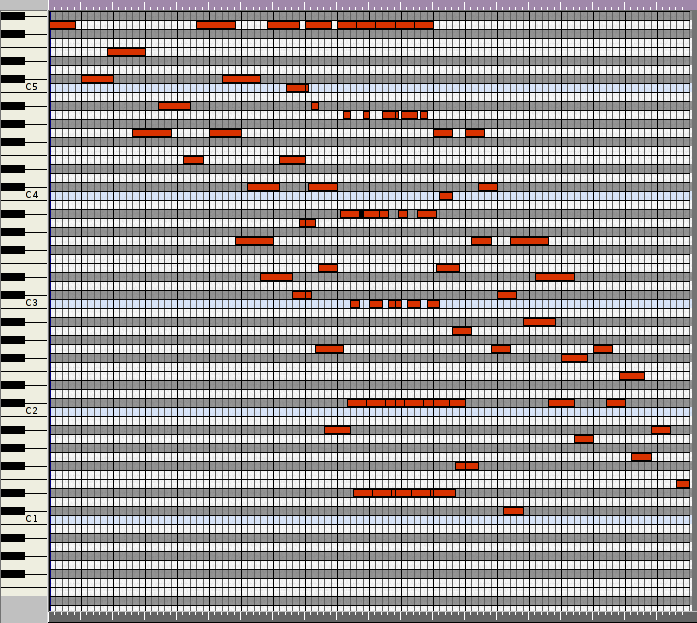
\includegraphics[scale=.5]{piano-roll-secao-2}
  \caption{Representação da amplitude na seção 2 em \eng{piano roll}}
  \label{fig:amplitude-secao-2}
\end{figure}

\begin{figure}
  \centering
  \includegraphics{secao-2}
  \caption{Redução analítica da seção 2---notas}
  \label{fig:notas-secao-2}
\end{figure}

A seção 3 compreende uma textura de melodia principal e
acompanhamento. A sua textura contém três elementos que podem ser
vistos na figura \ref{fig:textura-secao-3}: a) linha com notas de
articulação stacattíssimo atacadas nos tempos 1 e 2 (trompa); b) linha
com notas de articulação stacatto repetidas nas partes fracas do tempo
(fagote); c) melodia principal (clarinete). O elemento ``a'' é
apresentado com as notas lá e sol, o elemento ``b'' com as notas lá,
sol, dó$\sharp$ e ré$\sharp$, e o elemento ``c'' é apresentado com as
notas do motivo $alpha$ (figura \ref{fig:motivo-alfa}) com e sem
transposição para mi. O gestual da seção delineia um gradual aumento
de densidade e direcionamento para o agudo e culmina no início da
seção 4.

\begin{figure}
  \centering
  \includegraphics{textura-secao-3}
  \caption{Textura da seção 3}
  \label{fig:textura-secao-3}
\end{figure}

O início da seção 4 ocorre antes do final da seção 3, que tem um
desfecho gradativo, formando uma espécie de dégradé entre estas seções
(figura \ref{fig:transicao-secao-3-4}). A seção 4 é um fugato com
sujeito e contra-sujeito derivados do contorno principal e de
combinações de operações\footnote{Para maiores detalhes sobre este
  fugato e combinações de operações vide seção
  \ref{sec:comb-de-oper}.}. Do ponto de vista gestual, há uma passagem
de uma menor densidade no início da seção 4, com as entradas
instrumentais sucessivas, para uma maior densidade no final da mesma
seção. Isto ocorre por três razões: (1) a entrada da trompa em ritmo
largo (comp. 123), (2) o estreitamento entre as entradas das madeiras,
e (3) a partir do compasso 128, o jogo de perguntas e respostas com o
primeiro segmento do sujeito, que ocorre entre as duplas flauta/fagote
e oboé/clarinete.

\begin{figure}
  \centering
  \includegraphics{transicao-secao-3-4}
  \caption{Transição entre seções 3 e 4}
  \label{fig:transicao-secao-3-4}
\end{figure}

A seção 5 tem como elemento fundamental um ostinato na linha do fagote
(figura \ref{fig:ostinato-fagote}). Este ostinato é inspirado em um
dos toques da capoeira\footnote{A utilização deste elemento foi apenas
  pontual. Por este motivo não aprofundarei em maiores explicações
  sobre a capoeira e seus toques.}. O ritmo do ostinato é aproveitado
para a construção da estrutura de duas vozes (vide seção
\ref{sec:aspectos-verticais}). O desenho gestual desta seção é
bastante parecido ao da seção 1, com aumento progressivo da densidade
culminando no acorde do compasso 172.

\begin{figure}
  \centering
  \includegraphics{ostinato-fagote}
  \caption{Ostinato da linha do fagote}
  \label{fig:ostinato-fagote}
\end{figure}

A seção 6, em contraste às anteriores, é caracterizada por grupos de
notas curtas, rápidas e desligadas. Estes grupos são separados entre
si por silêncios (figura \ref{fig:sexta-secao-184-187}). As linhas dos
instrumentos contêm cada uma o motivo $\alpha$ modificado por
operações de rotação\footnote{Estas operações estão descritas na seção
  \ref{sec:comb-de-oper}.}. Os grupos de notas curtas não englobam
necessariamente todas as notas do motivo $\alpha$. Por vezes o
silêncio interrompe o motivo, como por exemplo na linha da flauta, nos
compassos 177--178 (figura \ref{fig:grupos-separados-silencio}). O
motivo é concluído logo após o silêncio.

\begin{figure}
  \centering
  \subfloat[Textura de notas curtas e silêncios (em dó)]{
    \includegraphics{sexta-secao-184-187}
    \label{fig:sexta-secao-184-187}
  }

  \subfloat[Motivo interrompido por silêncio]{
    \includegraphics{flauta-grupos-silencio}
    \label{fig:grupos-separados-silencio}
  }

  \subfloat[Transição entre os dois gestos da seção 6]{
    \includegraphics{transicao-sexta-dois-gestos}
    \label{fig:transicao-sexta-dois-gestos}
  }
  \caption{Notas curtas separadas por silêncios (seção 6)}
  \label{fig:sexta-secao-notas-curtas}
\end{figure}

A seção 6 contém dois gestos interligados. O primeiro gesto
(comp. 173--198) é marcado pelo aumento da densidade, obtido pela
diminuição dos silêncios. O colorido melódico tem destaque no final
deste gesto (comp. 194--198). O segundo gesto (comp. 199--214) é
caracterizado por graduais movimentos ascendentes e movimentação do
âmbito do grave para o agudo. A linha da trompa (comp. 206--215),
derivada da linha do oboé (comp. 149--157) interliga esta seção com a
seguinte. Na figura \ref{fig:transicao-sexta-dois-gestos} é possível
perceber o início do segundo gesto com elementos do gesto anterior.

A seção 7, última da obra, engloba elementos importantes das seções
anteriores (figura \ref{fig:setima-secao-resumo}). A linha do fagote é
uma repetição do que ocorre na seção 4. A linha do clarinete
representa o ritmo e acentuação da seção 3. A linha da trompa
corresponde ao solo do fagote do início da peça. As linhas do oboé e
flauta representam a estrutura de duas vozes apresentada na seção
5. Finalmente o material apresentado pela flauta e oboé a partir do
compasso 239 representa o sujeito do fugato da seção 4. As relações de
contornos nesta seção são, portanto, as mesmas que estes citados
elementos mantêm nas seções anteriores.

\begin{figure}
  \centering
  \includegraphics{setima-secao-resumo}
  \caption{Elementos de outras seções na seção 7}
  \label{fig:setima-secao-resumo}
\end{figure}
\section{Aspectos verticais}
\label{sec:aspectos-verticais}
%% aspectos "harmônicos". melhorar título da seção

A estrutura de duas vozes (figura \ref{fig:bifonia},
p. \pageref{fig:bifonia}) que origina todo material da peça tem seu
conteúdo harmônico derivado da escala octatônica\footnote{A escala
  octatônica é obtida a partir da superposição de duas das três
  tétrades diminutas contidas em uma escala dodecafônica
  \cite[p. 76]{antokoletz90:music}.} (figura
\ref{fig:escala-octatonica}).

\begin{figure}
  \centering
  \includegraphics{escala-octatonica}
  \caption{Escala octatônica}
  \label{fig:escala-octatonica}
\end{figure}

Ao longo da obra um acorde é apresentado de forma recorrente (figura
\ref{fig:acorde-motivo}). Este acorde é derivado da estrutura de duas
vozes e tem sonoridade octatônica. A seção 3 é inteiramente construída
com este acorde, que tem sua orquestração modificada no decorrer do
gesto.

\begin{figure}
  \centering
  \includegraphics{acorde-motivo}
  \caption{Acorde-motivo}
  \label{fig:acorde-motivo}
\end{figure}

A estrutura de duas vozes é apresentada em sua forma mais explícita na
seção 5 (figura \ref{fig:bifonia-grave}). Aparece inicialmente na
região grave, nas linhas do clarinete e da trompa (comp. 137--144),
depois brevemente no oboé e na trompa (comp. 146--149), e mais adiante
na flauta e no clarinete (comp. 157--172).

\begin{figure}
  \centering
  \includegraphics{bifonia-grave}
  \caption{Apresentação da estrutura de duas vozes no clarinete e
    trompa (ambos em dó) c. 137--141}
  \label{fig:bifonia-grave}
\end{figure}
\section{Uso de motivos}
\label{sec:uso-de-motivos}

A obra contém três motivos derivados da estrutura de duas vozes
(figura \ref{fig:bifonia}, p. \pageref{fig:bifonia}). O motivo
$\alpha$ (figura \ref{fig:motivo-alfa-analisado}) dá origem aos
motivos de três notas $\beta$ (figura \ref{fig:motivo-beta}) e de
semicolcheias $\gamma$ (figura \ref{fig:motivo-gama}). Além destes há
a presença de um motivo unicamente rítmico $\delta$ (figura
\ref{fig:motivo-delta}).

\begin{figure}
  \centering
  \subfloat[Motivo $\beta$]{
    \includegraphics{motivo-beta}
    \label{fig:motivo-beta}
  }
  \subfloat[Motivo $\gamma$]{
    \includegraphics{motivo-gama}
    \label{fig:motivo-gama}
  }

  \subfloat[Motivo $\delta$]{
    \includegraphics{motivo-delta}
    \label{fig:motivo-delta}
  }

  \subfloat[Estrutura do motivo $\alpha$]{
    \includegraphics{motivo-alfa-analisado}
    \label{fig:motivo-alfa-analisado}
  }
  \caption{Motivos utilizados na obra}
  \label{fig:motivos-utilizados}
\end{figure}

O motivo $\alpha$ contém dois motivos $\beta$, um em sua forma
original e outro invertido. Além disso o motivo $\alpha$ também está
presente de forma invertida no motivo $\gamma$, com as notas
Dó-Mi$\flat$-Ré$\flat$. Este motivo $\alpha$ é utilizado na linha do
fagote do início da peça, no sujeito do fugato da seção 4 (letra L),
na linha do clarinete nos compassos 137--144, na linha da flauta nos
compassos 158--171, no material da flauta e oboé na seção 6 (letra R)
e na seção final.
%% inserir figura com linha inicial do fagote
%% inserir seção em que falo que a última seção é resumo das outras

O motivo $\gamma$ é exatamente um retrógrado do motivo $\alpha$ com a
adição do parâmetro duração e da característica anacrúzica. O motivo
está presente na linha do oboé, compasso 149, nas linhas da flauta e
clarinete nos compassos 157--172, na contrução do material ascendente
dos compassos 200--215 e na seção final.

O motivo $\delta$ não tem relação com altura ou contorno. É apenas um
padrão de acentuação que é repetido nas seções 3 e 7. Na primeira
aparição há notas \eng{stacatto} entre os acentos. Na segunda aparição
há apenas os acentos.

\section{Uso de contornos}
\label{sec:uso-de-contornos}

O objetivo principal da composição da obra \obra{} foi o uso
sistemático de combinações de operações de contorno para a criação
musical. Por isso decidi escolher um único contorno---de modo a
colaborar com a unidade da peça---e manipulá-lo para gerar a maioria
do material composicional da obra. Escolhi o contorno de seis
elementos \contpr{}, relacionado com a estrutura de duas vozes e o
motivo $\alpha$.

O contorno principal \contpr{} tem forma prima c6-26 (0 2 1 4 3
5)\footnote{A numeração dos contornos (ou segmentos de contornos) pode
  ser vista na Tabela de classes de segmentos de contornos
  \cite{marvin.ea87:relating}.}. Este é um contorno simétrico, por
isso retrógrado e inversão são iguais. Este contorno contém
subconjuntos de 5, 4, 3 e 2 elementos.

\subsection{Combinações de operações de contorno utilizadas}
\label{sec:comb-de-oper}

Utilizei um grupo de operações de contorno e as combinei para criar o
material musical da obra. Trabalhei com dois subconjuntos de
contornos, operações de int$_1$, inversão, rotações e de preenchimento
de contornos. Combinei estas operações desta forma:

\begin{itemize}
\item Subconjunto com expansão e transposição
\item Interpolação com expansão
\item Rotação com expansão
\item Concatenação de contornos resultando em novo material
\item Rotação com retrogradação
\end{itemize}

%% dúvida: que termo devo usar em relação à linha do fagote? melodia?
%% fragmento melódico? motivo?

%% kroger: talvez "solo de fagote" se voce esta se referindo apenas ao
%% solo de fagote (antes dos instrumentos entrarem) :-)

%% marcos: estou preferindo deixar "melodia"

A combinação das operações de subconjunto, expansão e transposição foi
utilizada na linha do fagote no início da peça. Neste ponto há uma
melodia (figura \ref{fig:melodia-inicial},
p. \pageref{fig:melodia-inicial}) construída com o subconjunto do
contorno principal (2 0 1). A melodia tem dois segmentos, sendo o
primeiro derivado das três notas iniciais do motivo $\alpha$, e o
segundo como transposição do segmento anterior com operações de
expansão e transposição. Em ambos os segmentos há preservação do
contorno (2 0 1). Esta melodia está presente em toda a primeira seção
da obra, nos compassos 9--14 no fagote e oboé, nos compassos 15--22 no
clarinete, e nos compassos 23--36 na flauta e trompa.

A combinação de rotação e expansão de contornos ocorre no sujeito e
contra-sujeito do fugato da seção 4 e no material de notas curtas da
seção 6. O sujeito do fugato (figura \ref{fig:sujeito-fugato}) é
constituído por dois segmentos elididos. O primeiro segmento é o
próprio motivo $\alpha$, por consequüencia, é também o contorno
principal (5 3 4 1 2 0). O segundo segmento é o contorno resultante da
combinação da operação de rotação de fator 3, (1 2 0 5 3 4), e da
operação de expansão. O segundo segmento é iniciado na nota Sol,
última nota do segmento anterior.

O contra-sujeito é composto de três segmentos que contêm combinações
de operações de retrogradação e rotação de contornos (figura
\ref{fig:contra-sujeito-fugato}). O primeiro segmento contém uma
rotação de fator 5 do retrógrado do contorno principal (5 0 2 1 4
3). A primeira nota está elidida com a última nota do sujeito. O
segundo segmento contém uma rotação de fator 4 do retrógrado do
contorno principal (3 5 0 2 1 4), e também está elidida ao segmento
anterior. Finalmente o terceiro segmento contém uma rotação de fator 3
do retrógrado do contorno principal (4 3 5 0 2 1). Ao contrário dos
outros segmentos, ele não está elidido ao segmento anterior. Pode-se
observar que o contra-sujeito incorpora ainda uma sistemática nas suas
operações de contorno. A cada segmento o fator de rotação diminui em
um ponto.

\begin{figure}
  \centering
  \subfloat[Sujeito]{
    \includegraphics{sujeito-fugato}
    \label{fig:sujeito-fugato}
  }

  \subfloat[Contra-Sujeito]{
    \includegraphics{contra-sujeito-fugato}
    \label{fig:contra-sujeito-fugato}
  }
  \caption{Elementos estruturais do fugato}
  \label{fig:elementos-fugato}
\end{figure}

A combinação de rotação e expansão de contornos também está presente
na seção 6, nas linhas das quatro madeiras. A linha da flauta contém o
motivo $\alpha$ em sua forma original. A linha do clarinete contém uma
rotação de fator 2 e uma expansão de intervalos de segunda para
intervalos de terça. A linha do oboé contém um desvio da estrutura do
contorno. Trata-se de uma rotação de fator 3 do motivo $\alpha$, porém
com transposição da segunda metade do motivo para uma oitava
abaixo. Neste ponto a estrutura do contorno foi sacrificada em prol do
desenho gestual da seção, que não supera o Ré$\sharp$4 neste
trecho. Finalmente a linha do fagote contém uma rotação de fator 4 do
motivo $\alpha$ e expansão semelhante ao do clarinete. Na figura
\ref{fig:notas-curtas-madeiras} estão exibidas estas variações do
motivo $\alpha$ em cada elemento, na tabela
\ref{tab:operacoes-secao-6} há um esquema com as operações utilizadas
nestas variações, e na figura \ref{fig:rotacoes-534120} estão
representações gráficas das rotações utilizadas.

\begin{figure}
  \centering
    \includegraphics{notas-curtas-madeiras}
    \caption{Operações de rotação e expansão do motivo $\alpha$ na 6ª
    seção}
  \label{fig:notas-curtas-madeiras}
\end{figure}

\begin{figure}
  \centering
  \subfloat[Rotação 2: (4 1 2 0 5 3)]{
    \includegraphics{c-412053}
    \label{fig:412053}  
  }
  \subfloat[Rotação 3: (1 2 0 5 3 4)]{
    \includegraphics{c-120534}
    \label{fig:120534}  
  }
  \subfloat[Rotação 4: (2 0 5 3 4 1)]{
    \includegraphics{c-205341}
    \label{fig:205341}  
  }
  \caption{Rotações no contorno (5 3 4 1 2 0)}
  \label{fig:rotacoes-534120}
\end{figure}

\begin{table}
  \centering
  \begin{tabular}{r|cc}
    Instrumento & Fator de rotação & Expansão \\
    \hline
    Flauta & 0 & Não \\
    Oboé & 3 & Não \\
    Clarinete & 2 & Sim \\
    Fagote & 4 & Sim \\
  \end{tabular}
  \caption{Operações na seção 6}
  \label{tab:operacoes-secao-6}
\end{table}

A combinação entre expansão e retrogradação ocorre na linha do oboé
nos compassos 149--157 (figura \ref{fig:oboe-solo-secao-5}). O motivo
$\gamma$ (vide seção \ref{sec:uso-de-motivos} e figura
\ref{fig:motivo-gama}) é uma retrogradação do motivo $\alpha$ da
peça. Neste trecho este motivo aparece três vezes: na primeira vez em
sua forma original, na segunda vez com uma expansão e intervalo de
segunda para intervalo de terça, e na terça com uma expansão de
intervalo de segunda para intervalo de quarta.

%% inserir análise no inkscape
\begin{figure}
  \centering
  \includegraphics{oboe-solo-secao-5}
  \caption{Solo do oboé na seção 5}
  \label{fig:oboe-solo-secao-5}
\end{figure}

A combinação entre expansão, rotação, retrógrado e interpolação de
contornos ocorre na linha do oboé nos compassos 149--153. O motivo
$\alpha$ tem uma rotação de fator 3 gerando as notas adjacentes
Sol-Si$\flat$-Lá, e logo após, no compasso 152,
Dó$\sharp$-Si$\sharp$-Ré$\sharp$. Entre estes dois grupos de notas há
uma expansão de intervalos do motivo $\gamma$, iniciado em Dó$\sharp$3
e concluído em Dó$\sharp$4. Como já foi dito, este motivo é uma
retrogradação do motivo $\alpha$. Entendo que este motivo está
interpolado com o contorno iniciado em Sol.

\subsection{Operações de contornos não combinadas}
\label{sec:cont-nao-comb}

A operação de int$_1$ do contorno principal (- + - + -) ocorre de
maneira não ortodoxa no ostinato da linha do fagote, ao longo de toda
a seção 5 (figura \ref{fig:ostinato-fagote},
p. \pageref{fig:ostinato-fagote}). O padrão com as notas Sol e Lá
sugere o movimento (- +) presente no contorno principal.

A operação de expansão de intervalos também é usada de forma isolada
na segunda seção da obra. A expansão dos intervalos está associada à
omissão de notas da escala octatônica na construção do
contorno. Considerando-se a escala
Sol-Fá$\sharp$-Mi-Ré$\sharp$-Dó$\sharp$-Dó-Si$\flat$-Lá e omitindo-se
uma a cada duas notas, partindo-se de Sol tem-se
Sol-Mi-Dó$\sharp$-Si$\flat$. Omitindo-se duas a cada três notas tem-se
Sol-Ré$\sharp$-Si$\flat$ e assim por diante. O contorno é construído
com estas notas. A figura \ref{fig:escala-secao-2-one} mostra o
contorno com a omissão de uma a cada duas notas da escala octatônica,
e a figura \ref{fig:escala-secao-2-two} com a omissão de duas a cada
três notas da mesma escala.

\begin{figure}
  \centering
  \subfloat[Omissão de uma a cada duas notas]{
    \includegraphics[scale=1]{escala-secao-2-one}
    \label{fig:escala-secao-2-one}
  }

  \subfloat[Omissão de duas a cada três notas]{
    \includegraphics[scale=1]{escala-secao-2-two}
    \label{fig:escala-secao-2-two}
  }
  \caption{Expansão de intervalos por omissão de notas da escala
    octatônica}
  \label{fig:escala-secao-2}
\end{figure}

A operação de redução de contornos pode ser vista nas melodias
principais da seção 3 (figura \ref{fig:reducao-contornos-secao-3}). No
compasso 68 o contorno principal \contpr{} aparece na linha do
clarinete com apenas sua primeira e última notas (5 0). Nos compassos
76 e 81 o contorno aparece respectivamente nas linhas do oboé e
clarinete com apenas 4 notas. Na linha do oboé as notas centrais (4 1)
são omitidas para resultar no contorno (5 3 2 0), e na linha do
clarinete a segunda e penúltima notas (3 2) são omitidas para resultar
no contorno (5 4 1 0).

\begin{figure}
  \centering
  \subfloat[Nota inicial e nota final]{
    \includegraphics{reducao-contornos-secao-3-clarinete}
    \label{fig:reducao-contornos-secao-3-clarinete}
  }

  \subfloat[Omissão das duas notas centrais]{
    \includegraphics{reducao-contornos-secao-3-oboe}
    \label{fig:reducao-contornos-secao-3-oboe}
  }

  \subfloat[Omissão de duas notas intermediárias]{
    \includegraphics{reducao-contornos-secao-3-clarinete-2}
    \label{fig:reducao-contornos-secao-3-clarinete-2}
  }

  \caption{Redução de contornos na seção 3}
  \label{fig:reducao-contornos-secao-3}
\end{figure}

%% falar sobre o gestual da seção 5 e uso da anacruze e da
%% semelhança com o contraponto da primeira seção

\subsection{Contornos associados a outros parâmetros musicais}
\label{sec:cont-assoc-outr}

Contornos estão associados a outros parâmetros musicais como
andamento, densidade e textura.

Os andamentos utilizados na peça---82, 66, 120, 108 e 112 (vide tabela
\ref{tab:secoes-obra}, p. \pageref{tab:secoes-obra})---representam o
contorno A(1 0 4 2 3). Este contorno é um subconjunto de 5 elementos
do contorno principal utilizado, \contpr{}.

Na seção 1 relações de contornos estão associados a densidade. A
densidade neste trecho tem contorno D(1 3 2 5 4), isto é começa com um
instrumento, depois um trio, um duo, o quinteto completo e um
quarteto. Esta seção é iniciada com um solo de fagote (1) seguido de
um trio com fagote, clarinete e oboé (3). Ocorre então um duo entre
clarinete e flauta (2), um \eng{tutti} (5) e finalmente um quarteto
sem o fagote (4). Este contorno D é o retrógrado de um subconjunto de
5 elementos do contorno principal P.

As texturas presentes na peça podem ser divididas em dois grandes
grupos: de texturas homofônicas, que engloba texturas corais e de
melodia acompanhada; e de texturas polifônicas, que engloba textura
contrapontística e textura complexa. Estes grupos são apresentados
nesta ordem:
polifonia-homofonia-polifonia-homofonia-polifonia-homofonia. Considerando
que uma textura polifônica é mais complexa que uma textura homofônica,
a alternância entre estas texturas delineia um contorno de int$_1$ (-
+ - + -), derivado do contorno principal \contpr{}.

\chapter{Partitura da obra \obra{}}
\label{cha:partitura-da-obra}

\input{paginas-composicao}

\chapter{Conclusão e discussão}
\label{cha:conclusao-e-discussao}

Contornos são estruturas musicais que podem efetivamente colaborar com
a coerência de uma obra musical. Teóricos desenvolveram operações de
comparação para análise musical algumas das quais podem ser utilizadas
na criação de material composicional, conforme mostrei ao longo deste
trabalho. Estas operações podem ser combinadas e resultar em uma maior
variedade de elementos derivados de um mesmo material gerador.

A obra \obra{} apresenta diversos usos de operações de contornos e
combinações. Toda obra foi desenvolvida a partir do contorno \contpr{}
e reuniu um grupo de operações e combinações derivadas de teorias de
contorno. Uma vez que há uma carência de literatura sobre contornos na
composição este estudo contribui de forma significativa com a
ampliação do estado de arte de teorias de contorno incorporando
possibilidades de aplicações de operações de contorno na composição
musical.

% operações "mais e menos interessantes"

Das operações de contorno experimentadas algumas foram vistas como
mais adequadas para a composição musical, como expansão e redução de
intervalos, retrogradação, inversão, rotação, subconjuntos, rotação e
concatenação. No entanto outras operações desenvolvidas para análise
não pareceram funcionais para a criação musical. A matriz de
comparação por exemplo, embora tenha sido intensamente usada por
Morris, Marvin e Laprade, não parece ter um uso interessante para
composição.

A realização deste estudo abre caminho para vários outros trabalhos.

% Expansão do estudo: mapeamento de parâmetros em função de outros
% parâmetros além do tempo, survey

É importante fazer um mapeamento dos mais diversos parâmetros musicais
como dinâmica, densidade ou textura em função de outros parâmetros
além do tempo. Desta forma pode-se trabalhar com contornos como
dinâmica em função da densidade ou homogeneidade de timbre em função
da complexidade rítmica.

% Utilização de outras operações em composição.

É interessante testar outras operações das teorias de contornos em
composição compondo estudos de forma sistemática para testar cada
operação. Dessa forma é possível realmente saber como cada operação
pode ser utilizada na criação musical.

É importante compor estudos com instrumentos mais variados, como por
exemplo instrumentos sintetizados por computador. Este estudo pode
contribuir com os trabalhos de música computacional disponibilizando
contorno como elemento estruturador.

% Expansão do Goiaba

É necessário expandir o software Goiaba inserindo operações de todas
as teorias de contorno, acrescentando uma interface gráfica para que o
usuário possa clicar e arrastar pontos em um gráfico para gerar
contornos, inserindo funções para gerar partituras a partir de
contornos, e criando uma versão multiplataforma. Este estudo, além de
representar uma significativa ferramenta para a área de Composição,
pode incentivar compositores a usarem contornos de forma sistemática
em suas obras.

%%% Local Variables: 
%%% mode: latex
%%% TeX-master: "dissertacao-default"
%%% End: 
\bibliographystyle{plain}
\nocite{houaiss.ea01:dicionario,nienhuys.ea08:lilypond,seibel05:practical,graham94:lisp,shapiro92:common,team07:sbcl,stallman07:gnu,team05:slime,leunen92:handbook}
\bibliography{melodic-contour,music-perception,composition,music-harmony-and-theory,programs,music-analysis,audio,dictionary,genos,computer-science,writing-style}

\end{document}
